%Version 3.1 December 2024
% See section 11 of the User Manual for version history
%
%%%%%%%%%%%%%%%%%%%%%%%%%%%%%%%%%%%%%%%%%%%%%%%%%%%%%%%%%%%%%%%%%%%%%%
%%                                                                 %%
%% Please do not use \input{...} to include other tex files.       %%
%% Submit your LaTeX manuscript as one .tex document.              %%
%%                                                                 %%
%% All additional figures and files should be attached             %%
%% separately and not embedded in the \TeX\ document itself.       %%
%%                                                                 %%
%%%%%%%%%%%%%%%%%%%%%%%%%%%%%%%%%%%%%%%%%%%%%%%%%%%%%%%%%%%%%%%%%%%%%

%%\documentclass[referee,sn-basic]{sn-jnl}% referee option is meant for double line spacing

%%=======================================================%%
%% to print line numbers in the margin use lineno option %%
%%=======================================================%%

%%\documentclass[lineno,pdflatex,sn-basic]{sn-jnl}% Basic Springer Nature Reference Style/Chemistry Reference Style

%%=========================================================================================%%
%% the documentclass is set to pdflatex as default. You can delete it if not appropriate.  %%
%%=========================================================================================%%

%%\documentclass[sn-basic]{sn-jnl}% Basic Springer Nature Reference Style/Chemistry Reference Style

%%Note: the following reference styles support Namedate and Numbered referencing. By default the style follows the most common style. To switch between the options you can add or remove �Numbered� in the optional parenthesis. 
%%The option is available for: sn-basic.bst, sn-chicago.bst%  
 
%%\documentclass[pdflatex,sn-nature]{sn-jnl}% Style for submissions to Nature Portfolio journals
%%\documentclass[pdflatex,sn-basic]{sn-jnl}% Basic Springer Nature Reference Style/Chemistry Reference Style
\documentclass[pdflatex,sn-mathphys-num]{sn-jnl}% Math and Physical Sciences Numbered Reference Style
%%\documentclass[pdflatex,sn-mathphys-ay]{sn-jnl}% Math and Physical Sciences Author Year Reference Style
%%\documentclass[pdflatex,sn-aps]{sn-jnl}% American Physical Society (APS) Reference Style
%%\documentclass[pdflatex,sn-vancouver-num]{sn-jnl}% Vancouver Numbered Reference Style
%%\documentclass[pdflatex,sn-vancouver-ay]{sn-jnl}% Vancouver Author Year Reference Style
%%\documentclass[pdflatex,sn-apa]{sn-jnl}% APA Reference Style
%%\documentclass[pdflatex,sn-chicago]{sn-jnl}% Chicago-based Humanities Reference Style

%%%% Standard Packages
%%<additional latex packages if required can be included here>

% \usepackage{graphicx}%
% \usepackage{multirow}%
\usepackage{amsmath,amssymb,amsfonts}%
\usepackage{amsthm}%
\usepackage{mathrsfs}%
% \usepackage[title]{appendix}%
% \usepackage{xcolor}%
% \usepackage{textcomp}%
% \usepackage{manyfoot}%
% \usepackage{booktabs}%
% \usepackage{algorithm}%
% \usepackage{algorithmicx}%
% \usepackage{algpseudocode}%
% \usepackage{listings}%

\usepackage{hyperref}

%%%% For camera-ready, use this
%\documentclass[sigconf]{aamas}

\usepackage{listings}
\usepackage{xcolor}

\definecolor{codegreen}{rgb}{0,0.6,0}
\definecolor{codegray}{rgb}{0.5,0.5,0.5}
\definecolor{codepurple}{rgb}{0.58,0,0.82}
\definecolor{backcolour}{rgb}{0.95,0.95,0.92}
 
\lstdefinestyle{mystyle}{
    backgroundcolor=\color{backcolour},   
    commentstyle=\color{codegreen},
    keywordstyle=\color{magenta},
    numberstyle=\tiny\color{codegray},
    stringstyle=\color{codepurple},
    basicstyle=\footnotesize,
    breakatwhitespace=false,         
    breaklines=true,                 
    captionpos=b,                    
    keepspaces=true,                 
    numbers=left,                    
    numbersep=5pt,                  
    showspaces=false,                
    showstringspaces=false,
    showtabs=false,                  
    tabsize=2
}
 
\lstset{style=mystyle}

% --- Tickz
\usepackage{physics}
\usepackage{tikz}
\usepackage{amsmath}
\usepackage{mathdots}
% \usepackage{yhmath}
\usepackage{cancel}
\usepackage{color}
\usepackage{siunitx}
\usepackage{array}
\usepackage{multirow}
% \usepackage{amssymb}
\usepackage{gensymb}
\usepackage{tabularx}
\usepackage{extarrows}
\usepackage{booktabs}
\usetikzlibrary{fadings}
\usetikzlibrary{patterns}
\usetikzlibrary{shadows.blur}
\usetikzlibrary{shapes}

% ---------

\usepackage{balance} % for balancing columns on the final page
\usepackage{csquotes}
% \usepackage{cite}
\newcommand{\probP}{\text{I\kern-0.15em P}}
\usepackage{etoolbox}
\patchcmd{\thebibliography}{\section*{\refname}}{}{}{}
% \usepackage{amsthm,amssymb,amsfonts}

\usepackage[T1]{fontenc}
\usepackage{graphicx}
\usepackage{color}
% \renewcommand\UrlFont{\color{blue}\rmfamily}

\usepackage[inline, shortlabels]{enumitem}
\usepackage{tabularx}
\usepackage{caption}
\usepackage{listings}
\usepackage{stfloats}
\usepackage{titlesec}
\usepackage{ragged2e}
% \usepackage[hyphens]{url}
\usepackage[linesnumbered,ruled,vlined]{algorithm2e}
\usepackage{float}
\usepackage[english]{babel}

%%%%

%%%%%=============================================================================%%%%
%%%%  Remarks: This template is provided to aid authors with the preparation
%%%%  of original research articles intended for submission to journals published 
%%%%  by Springer Nature. The guidance has been prepared in partnership with 
%%%%  production teams to conform to Springer Nature technical requirements. 
%%%%  Editorial and presentation requirements differ among journal portfolios and 
%%%%  research disciplines. You may find sections in this template are irrelevant 
%%%%  to your work and are empowered to omit any such section if allowed by the 
%%%%  journal you intend to submit to. The submission guidelines and policies 
%%%%  of the journal take precedence. A detailed User Manual is available in the 
%%%%  template package for technical guidance.
%%%%%=============================================================================%%%%

%% as per the requirement new theorem styles can be included as shown below
\theoremstyle{thmstyleone}%
\newtheorem{theorem}{Theorem}%  meant for continuous numbers
%%\newtheorem{theorem}{Theorem}[section]% meant for sectionwise numbers
%% optional argument [theorem] produces theorem numbering sequence instead of independent numbers for Proposition
\newtheorem{proposition}[theorem]{Proposition}% 
%%\newtheorem{proposition}{Proposition}% to get separate numbers for theorem and proposition etc.

\theoremstyle{thmstyletwo}%
\newtheorem{example}{Example}%
\newtheorem{remark}{Remark}%

\theoremstyle{thmstylethree}%
\newtheorem{definition}{Definition}%

\raggedbottom
%%\unnumbered% uncomment this for unnumbered level heads

\begin{document}

\title[Assisting Multi-Agent System Design with MOISE+ and MARL: The MAMAD Method]{Assisting Multi-Agent System Design with $\mathcal{M}OISE^+$ and MARL: The MAMAD Method}

%%=============================================================%%
%% GivenName	-> \fnm{Joergen W.}
%% Particle	-> \spfx{van der} -> surname prefix
%% FamilyName	-> \sur{Ploeg}
%% Suffix	-> \sfx{IV}
%% \author*[1,2]{\fnm{Joergen W.} \spfx{van der} \sur{Ploeg} 
%%  \sfx{IV}}\email{iauthor@gmail.com}
%%=============================================================%%

\author*[1]{\fnm{Julien} \sur{Soulé}}\email{julien.soule@lcis.grenoble-inp.fr}

\author[1]{\fnm{Jean-Paul} \sur{Jamont}}\email{jean-paul.jamont@lcis.grenoble-inp.fr}
% \equalcont{These authors contributed equally to this work.}

\author[1]{\fnm{Michel} \sur{Occello}}\email{michel.occello@lcis.grenoble-inp.fr}

\author[2]{\fnm{Louis-Marie} \sur{Traonouez}}\email{louis-marie.traonouez@thalesgroup.com}

\author[3]{\fnm{Paul} \sur{Théron}}\email{paul.theron@orange.fr}

\affil*[1]{\orgdiv{Laboratoire de Conception et d'Intégration des Systèmes (LCIS)}, \orgname{Université Grenoble Alpe}, \orgaddress{\street{50 Rue Barthélémy de Laffemas}, \city{Valence}, \postcode{26000}, \state{Auvergne-Rhône-Alpes}, \country{France}}}

\affil[2]{\orgdiv{Thales Land and Air Systems}, \orgname{BL IAS}, \orgaddress{\street{1 Rue Louis Braille}, \city{Saint-Jacques-de-la-Lande}, \postcode{35136}, \state{Ille-et-Vilaine}, \country{France}}}

\affil[3]{\orgname{AICA IWG}, \orgaddress{\street{22 Av. Gazan Prolongée, 06600 Antibes}, \city{Antibes}, \postcode{06600}, \state{Provence-Alpes-Côte d'Azur}, \country{France}}}

%%==================================%%
%% Sample for unstructured abstract %%
%%==================================%%

\abstract{
Designing Multi-Agent Systems (MAS) requires balancing structured behaviors with adaptability. Traditional Agent-Oriented Software Engineering (AOSE) relies on expert knowledge, while Multi-Agent Reinforcement Learning (MARL) enables autonomous learning but lacks interpretability and control.
%
To bridge this gap, we propose the \textbf{MOISE+MARL Assisted MAS Design (MAMAD)} method, integrating the organizational modeling principles of $\mathcal{M}OISE^+$ with MARL. MAMAD treats MAS design as an optimization problem under organizational constraints, enabling structured yet adaptable policies and introducing a novel evaluation framework for organizational alignment.
%
We validate MAMAD in four case studies: Cyber-Defense scenario, Warehouse Management, Predator-Prey, and Overcooked-AI. Results show improved coordination, stability, and interpretability while reducing reliance on manual design efforts. MAMAD proposes a systematic approach to scalable, learning-based MAS design.
}

% Introduction
% Purpose
% Methods
% Results
% Conclusion

\keywords{Agent-oriented Software Engineering, Multi-Agent Reinforcement Learning, Assisted-Design, Organizational Model}

%%\pacs[JEL Classification]{D8, H51}

%%\pacs[MSC Classification]{35A01, 65L10, 65L12, 65L20, 65L70}

\maketitle

\section{Introduction}

\subsection{Context}

Designing \textbf{Multi-Agent Systems (MAS)} for complex real-world applications, such as \textbf{cybersecurity}, \textbf{logistics}, \textbf{autonomous robotics}, and \textbf{intelligent transportation}, requires robust methodologies that ensure both \textbf{structured agent behaviors} and \textbf{efficient task execution}. Traditionally, the \textbf{Agent-Oriented Software Engineering (AOSE)} paradigm has provided systematic frameworks for specifying and developing MAS, emphasizing the design of agents, roles, and interactions~\cite{Pavon2003, Bernon2005}. AOSE methodologies typically rely on explicit knowledge representation and predefined organizational models to structure agent behavior, ensuring predictability, reliability, and adherence to system-wide constraints~\cite{Hindriks2014}.

However, traditional AOSE approaches have significant \textbf{limitations in adaptability and scalability}. They often require extensive domain expertise to define organizational structures and behavioral rules, making them difficult to generalize across dynamic environments. Moreover, AOSE-based MAS typically lack \textbf{learning capabilities}, restricting their ability to autonomously adapt to unforeseen changes in the operational context~\cite{Garcia2004}.

In contrast, \textbf{Multi-Agent Reinforcement Learning (MARL)} has emerged as a promising approach for enabling autonomous agents to \textbf{learn and adapt} through experience. MARL techniques allow agents to develop \textbf{coordination strategies} by interacting with their environment and optimizing their decision-making policies based on cumulative rewards~\cite{Zhang2021}. This data-driven learning paradigm enables agents to dynamically adjust their behaviors to different contexts, even in highly uncertain or complex environments such as decentralized control, adversarial scenarios, or cooperative problem-solving~\cite{Papoudakis2021}.

Despite its adaptability, MARL presents significant challenges in terms of \textbf{interpretability and control}. Unlike AOSE, which enforces structured agent interactions through predefined models, MARL relies on emergent behaviors, which can be unpredictable and difficult to interpret~\cite{Du2022}. This lack of transparency poses challenges in critical domains such as \textbf{cybersecurity} and \textbf{human-agent collaboration}, where ensuring explainability and adherence to high-level constraints is crucial. Furthermore, MARL lacks built-in mechanisms to enforce \textbf{organizational constraints}, such as predefined roles, team structures, or safety guidelines, limiting its applicability in mission-critical MAS applications~\cite{Nguyen2020}.

Given these contrasting advantages and limitations, a natural research question arises: \textbf{How can we integrate the structured modeling capabilities of AOSE with the adaptive learning potential of MARL to design effective MAS?} Answering this question requires a \textbf{new approach} that unifies the strengths of both paradigms, providing a systematic way to \textbf{design MAS while enabling agents to learn and adapt within organizational constraints}.

\subsection{Problem statement and research gaps}

To formalize this idea, we propose a \textbf{new perspective on MAS design}: we consider that designing a MAS in a deployment environment to achieve a global goal efficiently (while respecting additional user-defined requirements) can be formulated as an \textbf{optimization problem under constraints in a MARL context}. In this formulation:
\begin{itemize}
    \item The \textbf{variable to optimize} is the agents' joint policy in the policy space.
    \item The \textbf{objective function} is to maximize the cumulative reward over time.
    \item The \textbf{constraints} are the organizational specifications, such as user-defined roles and goals.
\end{itemize}
This new formulation serves as the backbone of this article and motivates our contribution.

Despite the advancements in AOSE and MARL, several key research gaps remain unaddressed when considering the design of MAS through an \textbf{organizational learning perspective}:

\begin{itemize}
    \item \textbf{(G1) Lack of a unified framework linking AOSE and MARL for MAS design}: Existing AOSE methodologies do not integrate learning mechanisms, and MARL approaches lack structured design constraints. There is no \textbf{unified framework that automates MAS design by leveraging both AOSE principles and MARL-based learning}~\cite{Cossentino2014}.
    
    \item \textbf{(G2) Lack of structured interpretability in emergent behaviors}: MARL agents often develop unpredictable strategies, making it difficult to understand and justify their behaviors. There is a need for a method to analyze \textbf{how emergent collective behaviors align with predefined organizational structures}~\cite{Du2022}.
    
    \item \textbf{(G3) Lack of a standardized evaluation of organizational alignment}: While some approaches assess agent coordination, they do not systematically evaluate \textbf{how well agents adhere to predefined organizational roles and missions}~\cite{Papoudakis2021}.
    
    \item \textbf{(G4) Lack of control over organizational alignment in learning-based MAS}: There is no mechanism to \textbf{guide agents toward structured behaviors while preserving learning flexibility}. Most MARL approaches prioritize performance optimization without enforcing \textbf{organizational constraints} that could enhance explainability and stability~\cite{Oroojlooy2023}.
    
    \item \textbf{(G5) Excessive reliance on expert knowledge in MAS design}: Current MAS design methods heavily depend on domain experts to define agent roles and interactions. This reduces scalability and generalizability, as manually crafted specifications \textbf{may not transfer well across different application domains}~\cite{Nguyen2020}.
\end{itemize}

These gaps motivate the need for a \textbf{new method that integrates organizational modeling into MARL-based MAS design}.

\subsection{Contributions and paper organization}

To address these gaps, we introduce the \textbf{MOISE+MARL Assisted MAS Design (MAMAD) method}, built upon the \textbf{MOISE+MARL} framework~\cite{soule2025moisemarl} to leverage \textbf{$\mathcal{M}OISE^+$}, a formal organizational model, to integrate structured design principles into MARL. This enables \textbf{controlled policy learning}, where agents are guided or constrained during training to align with predefined organizational specifications while also allowing for the extraction of refined organizational insights from emergent agent behaviors. By bridging \textbf{learning-based adaptability} with \textbf{organizational interpretability}, MAMAD provides a principled approach to designing MAS with structured yet adaptable policies. Our contributions are summarized as follows:

\begin{enumerate}
    \item We propose a \textbf{new paradigm for MAS design}, formulating it as an optimization problem in MARL under organizational constraints.
    \item We develop \textbf{MAMAD}, a method that leverages the \textbf{MOISE+MARL} framework to enforce structured roles and goals within MARL, ensuring controlled and interpretable learning.
    \item We introduce a \textbf{novel evaluation framework} that quantifies the organizational alignment of learned behaviors to help in refining suitable organizational design in a MAS.
    \item We conduct extensive experiments across four case studies (\textbf{Cyber-Defense, Warehouse Management, Predator-Prey, and Overcooked-AI}), demonstrating the impact of structured constraints on MAS design.
\end{enumerate}

The remainder of the paper is organized as follows. Section~\ref{sec:background} introduces the theoretical background, covering \textbf{Multi-Agent Reinforcement Learning (MARL)} and \textbf{$\mathcal{M}OISE^+$ organizational modeling}. Section~\ref{sec:related_works} discusses related works on MAS design, MARL, and organizational control. Section~\ref{sec:moise_marl} presents the \textbf{MOISE+MARL framework}, the foundation of our contribution. Section~\ref{sec:mamad} introduces the \textbf{MAMAD method}, detailing its design methodology. Section~\ref{sec:experimental_setup} describes the experimental setup, including evaluation metrics, case studies, and baselines. Section~\ref{sec:results} presents and analyzes experimental results, while Section~\ref{sec:conclusion} concludes with discussions on future research directions.

\section{Related works}\label{sec:related_works}

This section start tracing back works in AOSE field regarding assisting MAS design until transitioning to a more MARL perspective. Then, we explore works related to introducing organizational principles within MARL for design purposes

\subsection{An overview of AOSE methods for assisting design}

The field of AOSE has developed numerous methodologies for structuring, developing, and managing MAS. Traditional AOSE approaches, such as GAIA \cite{gaia1998}, ADELFE \cite{adelfe2002}, and INGENIAS \cite{ingenias2004}, have provided foundational frameworks that incorporate roles, interactions, and organizational models. While these methodologies offer robust structures, they largely depend on manual specification by experts, which can limit scalability and adaptability, particularly in dynamic environments.

In recent years, advancements in MARL have opened new possibilities for automating aspects of MAS design. MARL enables agents to autonomously learn behaviors that maximize their collective performance. However, despite its potential, MARL has been underutilized within AOSE methodologies for automating organizational aspects such as role allocation, mission inference, and organizational compliance.

Some research efforts have sought to bridge this gap. For example, Hammar \cite{hammar2019} has applied MARL to adapt policies dynamically in response to changing environments, but this work does not explicitly address how MARL could support AOSE's organizational needs. Thomas \cite{thomas2023} and Iocchi \cite{iocchi2023} have explored MARL frameworks in industrial MAS contexts, demonstrating their capacity for automating behavior adaptation and achieving specific goals. However, these studies do not fully integrate MARL within AOSE methodologies to facilitate role-based organizational design.

MAMAD builds on these advances by embedding the $\mathcal{M}OISE^+$ organizational framework into MARL, enabling an approach that can automate the design of MAS while adhering to organizational constraints. Previous AOSE methodologies such as KB-ORG \cite{kborg2001} have used templates to simplify organizational design, but they still require manual configuration. By contrast, MAMAD leverages MARL to infer roles and missions directly from agent behaviors, reducing the dependency on expert input and improving scalability.

Further, the use of $\mathcal{M}OISE^+$ within MAMAD adds another dimension to existing MARL applications by incorporating safety and interpretability constraints. Techniques such as Constrained Policy Optimization \cite{zhao2024} and Safe Exploration \cite{melcer2024} have addressed safety in MARL, but they do not focus on enforcing organizational rules, which are essential for interpretable and compliant agent behavior. Shielding techniques, like those introduced by ElSayed-Aly et al. \cite{elsayed2021}, have also focused on preventing unsafe actions, yet they do not provide a complete organizational structure as $\mathcal{M}OISE^+$ does.

Unlike \textit{AGR}~\cite{ferber2003} (Agent Group Role), which does not explicitly handle goals as an organizational specification, the $\mathcal{M}OISE^+$ model addresses both roles and goals. Roles can be seen as sets of behavioral rules that agents must follow when interacting with each other or their environment to achieve their global goals. In contrast, goals represent states that agents aim to reach without a predefined path, thus requiring autonomous learning mechanisms. We believe that goals complement roles by enhancing stability and adaptability.

In summary, MAMAD contributes to the AOSE and MARL fields by integrating these two areas in a way that enhances MAS design with automated, organization-aware learning capabilities. This integration not only addresses the need for scalable and adaptive MAS but also ensures that organizational rules and safety considerations are embedded in the learning process, making MAMAD a novel methodology that aligns with modern AOSE goals.

\subsection{An Overview of Organization within MARL for Design Purpose}

Ensuring that Multi-Agent Reinforcement Learning (MARL) aligns with predefined organizational structures is a key challenge for structured MAS design. This requires both \textbf{evaluating} how well learned behaviors conform to abstract organizational roles and \textbf{controlling} the learning process to guide agents toward desired organizational alignments. This section reviews relevant approaches related to these two aspects.

\subsubsection{Evaluating Organizational Fit}

Some works address role or goal inference to assess how well agents align with predefined structures or emergent coordination patterns.

Wilson et al.~\cite{wilson2008learning} propose a method for transferring roles in Multi-Agent Markov Decision Processes (MDPs), helping agents adapt by mapping roles across different environments. However, their model lacks abstraction, focusing on specific, task-related roles rather than broader organizational objectives.

Berenji and Vengerov~\cite{berenji2000learning} investigate coordination and role inference in UAV missions, enhancing cooperation by modeling agent dependencies. While useful for local cooperation, their approach remains task-specific and does not offer abstract role computation for evaluating organizational alignment.

Yusuf and Baber~\cite{yusuf2020inferential} employ inferential reasoning and Bayesian methods for dynamic task coordination among diverse agents. Their framework is effective for on-the-fly coordination but does not incorporate abstract role alignment with organizational principles.

Serrino et al.~\cite{serrino2019finding} examine dynamic role inference in social settings, where agents infer roles through interactions. Although their approach promotes flexible role adaptation, it focuses on operational roles rather than higher-level organizational structures.

\medskip

\noindent \textbf{Summary:} None of these works meet the requirements for abstract role computation or organizational fit evaluation. Our concept of organizational fit necessitates a framework that systematically assesses how agent behaviors align with predefined organizational goals.

\subsubsection{Controlling Organizational Fit}

Controlling organizational fit involves externally guiding MARL training to ensure learned policies adhere to organizational structures, typically through constraints or incentive mechanisms.

Achiam et al.~\cite{achiam2017cpo} introduce Constrained Policy Optimization (CPO), which adjusts agent policies under safety constraints while maximizing rewards. MOISE+MARL extends this idea by integrating organizational constraints beyond safety, shaping behavior toward predefined organizational expectations.

Ray et al.~\cite{ray2019benchmarking} propose Lagrangian-based approaches for balancing reward maximization with constraint satisfaction. Unlike these approaches, MOISE+MARL does not merely modify reward functions but dynamically adjusts action spaces to enforce constraint adherence at various levels, providing fine-grained control.

Safe exploration techniques ensure that agents learn while adhering to predefined constraints. Garcia et al.~\cite{garcia2015comprehensive} review methods for maintaining safe exploration, and Alshiekh et al.~\cite{alshiekh2018safe} propose shielding mechanisms to block unsafe actions. While shielding prevents harmful decisions, MOISE+MARL employs constraints to actively steer agents toward behaviors that align with organizational roles.

Hierarchical Reinforcement Learning (HRL) decomposes tasks into subtasks, aligning well with organizational hierarchies. Ghavamzadeh et al.~\cite{ghavamzadeh2006hrl} show that HRL improves coordination by structuring agent decision processes. MOISE+MARL takes a different approach by constraining MARL externally, maintaining a modular granularity while generating refined behaviors under organizational constraints.

Communication and coordination are crucial for achieving organizational fit, especially in large-scale MAS. Foerster et al.~\cite{foerster2018communication} propose decentralized coordination through shared knowledge, enabling distributed agents to cooperate without central control.

\medskip

\noindent \textbf{Summary:} Unlike HRL, MOISE+MARL stands out by incorporating external organizational constraints that influence agents within a standard MARL framework, enabling structured adaptation. Unlike Shielding or CPO, which focus primarily on safety constraints, MOISE+MARL utilizes action and reward modifications to enforce role alignment. By balancing flexibility and structure, MOISE+MARL enhances scalability and adaptability, simplifying user interactions by requiring only a minimal set of organizational specifications.



\section{The MOISE+MARL framework}\label{sec:moise_marl}

This section introduces the formalism used to describe the functioning framework of the MOISE+MARL framework.

\subsection{Markov framework for MARL}

To apply MARL techniques, we rely on the \textit{Decentralized Partially Observable Markov Decision Process} (Dec-POMDP)~\citep{Oliehoek2016}. This model is well-suited for MAS, as it models multiple agents in an uncertain environment. Unlike \textit{Partially Observable Stochastic Games} (POSG), the Dec-POMDP allows for a common reward function for agents, which promotes learning of collaborative actions~\citep{Beynier2013}.

A Dec-POMDP $d \in D$ (where $D$ is the set of Dec-POMDPs) is defined as a 7-tuple $d = (S, \{A_i\}, T, R, \{\Omega_i\}, O, \gamma)$, where $S = \{s_1,\dots,s_{|S|}\}$ is the set of possible states; $A_{i} = \{a_{1}^{i},\dots,a_{|A_{i}|}^{i}\}$ is the set of possible actions for agent $i$; $T$ represents the set of transition probabilities, with $T(s,a,s') = \probP(s'|s,a)$ as the probability of transitioning from state $s$ to state $s'$ following action $a$; $R: S \times A \times S \rightarrow \mathbb{R}$ is the reward function, assigning a reward based on the initial state, the action taken, and the resulting state; $\Omega_{i} = \{o_{1}^{i},\dots,o_{|\Omega_{i}|}^{i}\}$ is the set of possible observations for agent $i$; $O$ represents the set of observation probabilities, where $O(s',a,o) = \probP(o|s',a)$ is the probability of obtaining observation $o$ after performing action $a$ and reaching state $s'$; and $\gamma \in [0,1]$ is the discount factor, used to weight future rewards.


The following formalism is used with MOISE+MARL to solve the Dec-POMDP~\citep{Beynier2013,Albrecht2024}: $\mathcal{A}$ represents the set of $n$ \textbf{agents}; $\Pi$ denotes the set of \textbf{policies}, where a policy $\pi \in \Pi, \pi: \Omega \rightarrow A$ deterministically maps an observation to an action, representing the agent's internal strategy; $\Pi_{joint}$ represents the set of \textbf{joint policies}, with a joint policy $\pi_{joint} \in \Pi_{joint}, \pi_{joint}: \Omega^n \rightarrow A^n = \Pi^n$, which selects an action for each agent based on their respective observations, acting as a collection of policies used by agents within a team; $H$ is the set of \textbf{histories}, where a history (or trajectory) over $z \in \mathbb{N}$ steps (typically the maximum number of steps in an episode) is represented as the $z$-tuple $h = ((\omega_{k}, a_{k}) | k \leq z, \omega \in \Omega, a \in A)$, capturing successive observations and actions; $H_{joint}$ stands for the set of \textbf{joint histories}, with a joint history $h_{joint} \in H_{joint}$ over $z$ steps defined as the set of agent histories: $h_{joint} = \{h_1, h_2, \dots, h_n\}$; and finally, $V_{joint}(\pi_{joint}): \Pi_{joint} \rightarrow \mathbb{R}$ denotes the \textbf{expected cumulative reward} over a finite horizon (assuming $\gamma < 1$ or if the number of steps in an episode is finite), where $\pi_{joint}$ represents the joint policy for team $i$, with $\pi_{joint,-i}$ being the joint policies of other teams, considered as fixed.


% We refer to \textbf{solving the Dec-POMDP} as the search for a joint policy $\pi_{joint} \in \Pi_{joint}$ such that $\pi_{joint}s)$, achieving at least an expected cumulative reward of $s$, where $s \in \mathbb{R}$.

\subsection{The $\mathcal{M}OISE^+$ organizational model}

\begin{figure}[h!]
    \centering
    


\tikzset{every picture/.style={line width=0.75pt}} %set default line width to 0.75pt        

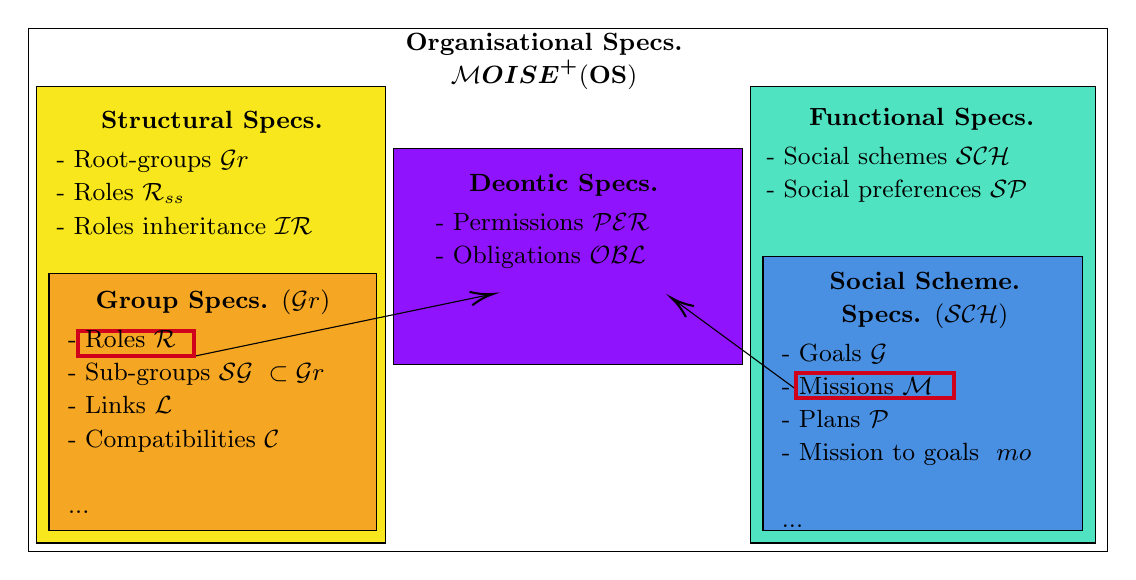
\begin{tikzpicture}[x=0.75pt,y=0.75pt,yscale=-1,xscale=1]
%uncomment if require: \path (0,1656); %set diagram left start at 0, and has height of 1656

%Shape: Rectangle [id:dp6756844921493015] 
\draw  [fill={rgb, 255:red, 248; green, 231; blue, 28 }  ,fill opacity=1 ] (46,1204) -- (214,1204) -- (214,1424) -- (46,1424) -- cycle ;
%Shape: Rectangle [id:dp3759944257810566] 
\draw  [fill={rgb, 255:red, 80; green, 227; blue, 194 }  ,fill opacity=1 ] (390,1204) -- (556,1204) -- (556,1424) -- (390,1424) -- cycle ;
%Shape: Rectangle [id:dp28244406216006945] 
\draw  [fill={rgb, 255:red, 144; green, 19; blue, 254 }  ,fill opacity=1 ] (218,1234) -- (386,1234) -- (386,1338) -- (218,1338) -- cycle ;
%Shape: Rectangle [id:dp32232123359581766] 
\draw   (42,1176) -- (562,1176) -- (562,1428) -- (42,1428) -- cycle ;
%Shape: Rectangle [id:dp7605706269262755] 
\draw  [fill={rgb, 255:red, 74; green, 144; blue, 226 }  ,fill opacity=1 ] (396,1286) -- (550,1286) -- (550,1418) -- (396,1418) -- cycle ;
%Shape: Rectangle [id:dp33110985390647496] 
\draw   (52,1294) -- (210,1294) -- (210,1418) -- (52,1418) -- cycle ;
%Shape: Rectangle [id:dp8653560038381976] 
\draw  [fill={rgb, 255:red, 245; green, 166; blue, 35 }  ,fill opacity=1 ] (52,1294) -- (210,1294) -- (210,1418) -- (52,1418) -- cycle ;
%Straight Lines [id:da09781093164567278] 
\draw    (412,1350) -- (353.61,1307.18) ;
\draw [shift={(352,1306)}, rotate = 36.25] [color={rgb, 255:red, 0; green, 0; blue, 0 }  ][line width=0.75]    (10.93,-3.29) .. controls (6.95,-1.4) and (3.31,-0.3) .. (0,0) .. controls (3.31,0.3) and (6.95,1.4) .. (10.93,3.29)   ;
%Straight Lines [id:da3938396723807833] 
\draw    (122,1334) -- (264.04,1304.41) ;
\draw [shift={(266,1304)}, rotate = 168.23] [color={rgb, 255:red, 0; green, 0; blue, 0 }  ][line width=0.75]    (10.93,-3.29) .. controls (6.95,-1.4) and (3.31,-0.3) .. (0,0) .. controls (3.31,0.3) and (6.95,1.4) .. (10.93,3.29)   ;
%Shape: Rectangle [id:dp269311335478327] 
\draw  [color={rgb, 255:red, 208; green, 2; blue, 27 }  ,draw opacity=1 ][line width=1.5]  (66,1322) -- (122,1322) -- (122,1334) -- (66,1334) -- cycle ;
%Shape: Rectangle [id:dp7449860119164387] 
\draw  [color={rgb, 255:red, 208; green, 2; blue, 27 }  ,draw opacity=1 ][line width=1.5]  (412,1342) -- (488,1342) -- (488,1354) -- (412,1354) -- cycle ;


% Text Node
\draw (472.5,1237.41) node   [align=left] {\begin{minipage}[lt]{112.2pt}\setlength\topsep{0pt}
\begin{center}
\textbf{{\small Functional Specs.}}
\end{center}
{\small  - Social schemes $\displaystyle \mathcal{SCH}$}\\{\small  - Social preferences $\displaystyle \mathcal{SP}$}
\end{minipage}};
% Text Node
\draw (474,1355) node   [align=left] {\begin{minipage}[lt]{103.36pt}\setlength\topsep{0pt}
\begin{center}
\textbf{{\small Social Scheme.}}\\{\small \textbf{Specs. }$\displaystyle (\mathcal{SCH})$}
\end{center}
{\small  - Goals $\displaystyle \mathcal{G}$}\\{\small  - Missions $\displaystyle \mathcal{M}$}\\{\small  - Plans $\displaystyle \mathcal{P}$}\\{\small  - Mission to goals \ $\displaystyle mo$}\\\\{\small  ...}
\end{minipage}};
% Text Node
\draw (131,1356) node   [align=left] {\begin{minipage}[lt]{104.72pt}\setlength\topsep{0pt}
\begin{center}
{\small \textbf{Group Specs. }$\displaystyle (\mathcal{G} r)$}
\end{center}
{\small  - Roles $\displaystyle \mathcal{R}$}\\{\small  - Sub-groups $\displaystyle \mathcal{SG} \ \subset \mathcal{G} r$}\\{\small  - Links $\displaystyle \mathcal{L}$}\\{\small  - Compatibilities $\displaystyle \mathcal{C}$}\\\\{\small  ...}
\end{minipage}};
% Text Node
\draw (181,1177) node [anchor=north west][inner sep=0.75pt]   [align=left] {\begin{minipage}[lt]{162.41pt}\setlength\topsep{0pt}
\begin{center}
{\small \textbf{Organisational Specs. }$\displaystyle \mathcal{M}\boldsymbol{OISE^{+}}$($\displaystyle \mathbf{OS}$)}
\end{center}

\end{minipage}};
% Text Node
\draw (300,1269.09) node   [align=left] {\begin{minipage}[lt]{92.48pt}\setlength\topsep{0pt}
\begin{center}
\textbf{{\small Deontic Specs.}}
\end{center}
{\small  - Permissions $\displaystyle \mathcal{PER}$}\\{\small  - Obligations $\displaystyle \mathcal{OBL}$}
\end{minipage}};
% Text Node
\draw (130.5,1245.69) node   [align=left] {\begin{minipage}[lt]{112.2pt}\setlength\topsep{0pt}
\begin{center}
\textbf{{\small Structural Specs.}}
\end{center}
{\small  - Root-groups $\displaystyle \mathcal{G} r$}\\{\small  - Roles $\displaystyle \mathcal{R}_{ss}$}\\{\small  - Roles inheritance $\displaystyle \mathcal{IR}$}
\end{minipage}};


\end{tikzpicture}
    \caption{A synthetic view of the $\mathcal{M}OISE^+$ model}
    \label{fig:moise_model}
\end{figure}

As illustrated in \autoref{fig:moise_model}, $\mathcal{M}OISE^+$ comprises three types of organizational specifications:

\noindent \paragraph{\textbf{Structural Specifications (SS)}} define how agents are structured to achieve goals, expressed as $\mathcal{SS} = \langle \mathcal{R}, \mathcal{IR}, \mathcal{G} \rangle$. $\mathcal{R}_{ss}$ is the set of roles ($\rho \in \mathcal{R}$) with an inheritance relation $\mathcal{IR}$ where $\rho_1 \sqsubset \rho_2$ if $\rho_1$ inherits from $\rho_2$. $\mathcal{GR}$ includes groups $\langle \mathcal{R}, \mathcal{SG}, \mathcal{L}^{intra}, \mathcal{L}^{inter}, \allowbreak \mathcal{C}^{intra}, \mathcal{C}^{inter}, np, ng \rangle$. Links ($\mathcal{L}$) define connections between roles: acquaintance, communication, or authority. Compatibilities $\mathcal{C}$ denote roles that agents can play together. Intra- and inter-group links and compatibilities are shown by $\mathcal{L}^{intra}$, $\mathcal{L}^{inter}$, $\mathcal{C}^{intra}$, and $\mathcal{C}^{inter}$, with $np$ and $ng$ defining role and subgroup counts.

\noindent \paragraph{\textbf{Functional Specifications (FS)}} describe the agents' goals, represented as $\mathcal{FS} = \langle \mathcal{SCH}, \mathcal{PO} \rangle$. The social scheme $\mathcal{SCH}$ includes global goals $\mathcal{G}$, missions $\mathcal{M}$, and plans $\mathcal{P}$ that organize goals in a tree structure. Plans link goals with an operator ($op$) indicating sequence, choice, or parallel completion. Missions map to goal sets ($mo$), and agent counts per mission are specified by $nm$. Preferences $\mathcal{PO}$ indicate which missions agents prefer, denoted as $m_1 \prec m_2$.

\noindent \paragraph{\textbf{Deontic Specifications (DS)}} indicate how structural specifications achieve functional goals, given by $\mathcal{DS} = \langle \mathcal{OBL}, \mathcal{PER} \rangle$. Time constraints $\mathcal{TC}$ set periods for permissions or obligations ($Any$ for any time). Obligations ($\mathcal{OBL}$) require agents in role $\rho_a$ to undertake mission $m$ at times $tc$, while permissions ($\mathcal{PER}$) allow it. The $rds$ function maps roles to their deontic specifications as $(tc, y, m)$ where $y$ distinguishes permission (0) from obligation (1).

\

\noindent Organizational specifications applied to agents are roles and goals (as missions) through permissions or obligations. Indeed, the other structural specifications such as compatibilities or links are inherent to roles. Similarly, we consider that the goals, the missions, and their mapping ($mo$) are enough to also link all of the other functional specifications such as plans, cardinalities, or preference orders.
Consequently, we consider it is sufficient to take into account roles, missions (goal and mapping) and permissions/obligations when linking $\mathcal{M}OISE^+$ with Dec-POMDP. 

\begin{figure*}[t]

    \label{eq:single_value_function}
    \raggedright
    \textbf{\textit{Définition 1} \quad Sate-Value function adapted to constraint guides in AEC mode:}

    \begin{scriptsize}
      \vspace{-0.3cm}
      \begin{gather*}
      V^{\pi^j}(s_t) = \hspace{-0.75cm} \sum_{\textcolor{red}{ \substack{a_{t} \in A \text{ si } rn() < ch_{t}, \\ 
      a_{t} \in A_{t} \text{ else}}
      }}{\hspace{-0.7cm} \pi_i(a_{t} | \omega_t)} \sum_{s_{t+1} \in S}\hspace{-0.1cm} T(s_{t+1} | s_t, a_{t})\Bigl[R(s_t,a_{t},s_{t+1}) + \\
      \hspace{2.7cm}\textcolor{blue}{ \sum_{m \in \mathcal{M}_i}{ \hspace{-0.1cm} v_m(t) \frac{grg_m(h_{t+1})}{1 - p + \epsilon} } } + \textcolor{red}{(1-ch_t) \times rrg(\omega_t,a_{t+1})} + V^{\pi^j_{i+1 \ mod \ n}}(s_{t+1})\Bigr]
    \end{gather*}  
    %
    \vspace{-0.3cm}
    %
    \textcolor{red}{$\hspace{0cm}\text{With } rag(h_t, \omega_t) = A_{t} \times \mathbb{R} \text{, } \langle a_t, ch_{t} \rangle \in A_{t} \times \mathbb{R} \text{ ; et } rn: \emptyset \to [0,1[ \text{, a uniform random function}$}
    %
    \vspace{-0cm}
    \textcolor{blue}{
    \begin{gather*}
    \hspace{0.1cm}{\text{With } \omega_t = O(\omega_t | s_t, a_t) \text{ ; } h_t = \{h_0 = \langle \rangle, h_{t+1} = \langle h_t, \langle \omega_{t+1}, a_{t+1} \rangle \rangle \} \text{ ; }} \\
    {grg_m(h) = \hspace{-0.8cm} \sum_{(grg_i,w_i) \in mo(m)}{\hspace{-0.8cm} w_i \times grg_i(h)} \text{ ; } \epsilon \in \mathbb{R}_{>0} \text{ ; }}
    \end{gather*}
    }
    \vspace{-1.05cm}
    \textcolor{blue}{
    \begin{gather*}
    \hspace{-0cm}
    v_m(t) = \{ 1 \text{ si } t \in t_c \text{ ; sinon } 0 \} \text{ ; et } \mathcal{M}_i = \{m_j \mid \langle ar(i),m_j,t_c,p \rangle \in \mathcal{M}\}
    \end{gather*}
    }
    \vspace{-0.6cm}

    \end{scriptsize}

\end{figure*}


\subsection{Linking $\mathcal{M}OISE^+$ with MARL}

\begin{figure}[h!]
    \centering
    \tikzset{every picture/.style={line width=0.75pt}} %set default line width to 0.75pt        

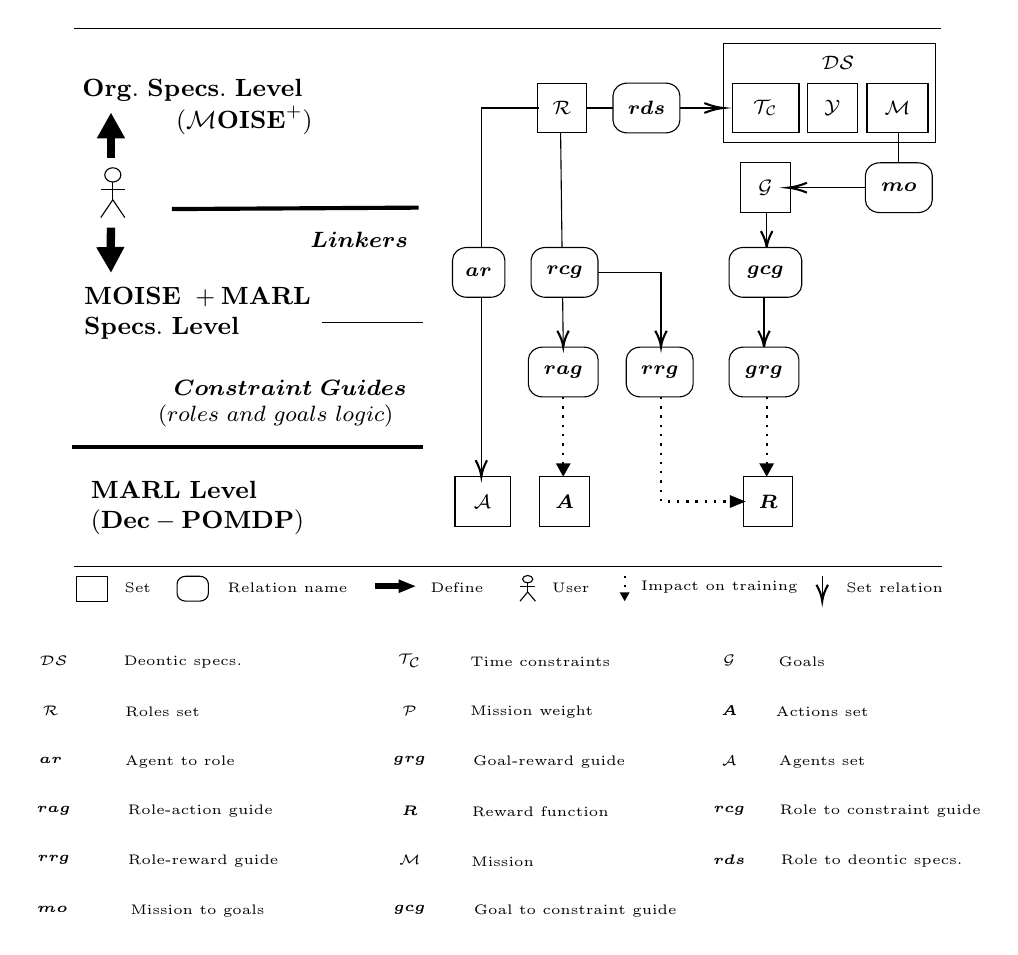
\begin{tikzpicture}[x=0.75pt,y=0.75pt,yscale=-1.2,xscale=1.4]
    %uncomment if require: \path (0,2584); %set diagram left start at 0, and has height of 2584

    %Straight Lines [id:da4973066741986565] 
    \draw [line width=1.5]    (118.21,2302.58) -- (203.1,2302) ;
    %Straight Lines [id:da14807114776731778] 
    \draw    (368.35,2272) -- (368.35,2294) -- (332.16,2294) ;
    \draw [shift={(330.16,2294)}, rotate = 360] [color={rgb, 255:red, 0; green, 0; blue, 0 }  ][line width=0.75]    (6.56,-1.97) .. controls (4.17,-0.84) and (1.99,-0.18) .. (0,0) .. controls (1.99,0.18) and (4.17,0.84) .. (6.56,1.97)   ;
    %Straight Lines [id:da16285043353898754] 
    \draw [line width=1.5]    (83.88,2398) -- (204.61,2398) ;
    %Straight Lines [id:da6299512000169913] 
    \draw    (169.94,2348) -- (204.61,2348) ;
    %Straight Lines [id:da64750232417664] 
    \draw    (84.65,2446) -- (383.15,2446) ;
    %Straight Lines [id:da35895220906699743] 
    \draw    (84.65,2230) -- (383,2230) ;
    %Straight Lines [id:da715014372569708] 
    \draw    (244.68,2262) -- (224.68,2262) -- (224.68,2408) ;
    \draw [shift={(224.68,2410)}, rotate = 270] [color={rgb, 255:red, 0; green, 0; blue, 0 }  ][line width=0.75]    (6.56,-1.97) .. controls (4.17,-0.84) and (1.99,-0.18) .. (0,0) .. controls (1.99,0.18) and (4.17,0.84) .. (6.56,1.97)   ;
    %Straight Lines [id:da71870438525014] 
    \draw    (251.96,2328) -- (286.51,2328) -- (286.51,2356) ;
    \draw [shift={(286.51,2358)}, rotate = 270] [color={rgb, 255:red, 0; green, 0; blue, 0 }  ][line width=0.75]    (6.56,-1.97) .. controls (4.17,-0.84) and (1.99,-0.18) .. (0,0) .. controls (1.99,0.18) and (4.17,0.84) .. (6.56,1.97)   ;
    %Straight Lines [id:da6006267784187092] 
    \draw [line width=0.75]  [dash pattern={on 0.84pt off 2.51pt}]  (252.87,2378) -- (252.87,2407) ;
    \draw [shift={(252.87,2410)}, rotate = 270] [fill={rgb, 255:red, 0; green, 0; blue, 0 }  ][line width=0.08]  [draw opacity=0] (5.36,-2.57) -- (0,0) -- (5.36,2.57) -- cycle    ;
    %Straight Lines [id:da8743336135156266] 
    \draw    (322.88,2304) -- (322.88,2316) ;
    \draw [shift={(322.88,2318)}, rotate = 270] [color={rgb, 255:red, 0; green, 0; blue, 0 }  ][line width=0.75]    (6.56,-1.97) .. controls (4.17,-0.84) and (1.99,-0.18) .. (0,0) .. controls (1.99,0.18) and (4.17,0.84) .. (6.56,1.97)   ;
    %Straight Lines [id:da14641229967966152] 
    \draw [line width=0.75]  [dash pattern={on 0.84pt off 2.51pt}]  (322.88,2378) -- (322.88,2407) ;
    \draw [shift={(322.88,2410)}, rotate = 270] [fill={rgb, 255:red, 0; green, 0; blue, 0 }  ][line width=0.08]  [draw opacity=0] (5.36,-2.57) -- (0,0) -- (5.36,2.57) -- cycle    ;
    %Straight Lines [id:da9260929933425808] 
    \draw [line width=0.75]  [dash pattern={on 0.84pt off 2.51pt}]  (286.51,2378) -- (286.51,2420) -- (312.61,2420) ;
    \draw [shift={(315.61,2420)}, rotate = 180] [fill={rgb, 255:red, 0; green, 0; blue, 0 }  ][line width=0.08]  [draw opacity=0] (5.36,-2.57) -- (0,0) -- (5.36,2.57) -- cycle    ;
    %Straight Lines [id:da3057006030233673] 
    \draw [line width=0.75]  [dash pattern={on 0.84pt off 2.51pt}]  (274,2449.7) -- (274,2457) ;
    \draw [shift={(274,2460)}, rotate = 270] [fill={rgb, 255:red, 0; green, 0; blue, 0 }  ][line width=0.08]  [draw opacity=0] (3.57,-1.72) -- (0,0) -- (3.57,1.72) -- cycle    ;
    %Straight Lines [id:da07288166228322246] 
    \draw    (342,2449.98) -- (342,2458) ;
    \draw [shift={(342,2460)}, rotate = 270] [color={rgb, 255:red, 0; green, 0; blue, 0 }  ][line width=0.75]    (6.56,-1.97) .. controls (4.17,-0.84) and (1.99,-0.18) .. (0,0) .. controls (1.99,0.18) and (4.17,0.84) .. (6.56,1.97)   ;
    %Shape: Ellipse [id:dp8508274348425935] 
    \draw   (95.09,2288.86) .. controls (95.09,2287.28) and (96.33,2286) .. (97.85,2286) .. controls (99.38,2286) and (100.62,2287.28) .. (100.62,2288.86) .. controls (100.62,2290.44) and (99.38,2291.71) .. (97.85,2291.71) .. controls (96.33,2291.71) and (95.09,2290.44) .. (95.09,2288.86) -- cycle ;
    %Straight Lines [id:da3825450168053828] 
    \draw    (97.85,2291.71) -- (97.85,2298.86) ;
    %Straight Lines [id:da521321206042058] 
    \draw    (97.85,2298.86) -- (93.71,2306) ;
    %Straight Lines [id:da055514206493922025] 
    \draw    (97.85,2298.86) -- (102,2306) ;
    %Straight Lines [id:da8996496708356774] 
    \draw    (102,2294.57) -- (93.71,2294.57) ;

    %Straight Lines [id:da31678488015771755] 
    \draw [line width=2.25]    (188,2454) -- (196.97,2454) ;
    \draw [shift={(201.97,2454)}, rotate = 180] [fill={rgb, 255:red, 0; green, 0; blue, 0 }  ][line width=0.08]  [draw opacity=0] (5.72,-2.75) -- (0,0) -- (5.72,2.75) -- cycle    ;
    %Shape: Ellipse [id:dp3927356466672782] 
    \draw   (238.88,2451.17) .. controls (238.88,2450.36) and (239.67,2449.7) .. (240.64,2449.7) .. controls (241.61,2449.7) and (242.4,2450.36) .. (242.4,2451.17) .. controls (242.4,2451.99) and (241.61,2452.65) .. (240.64,2452.65) .. controls (239.67,2452.65) and (238.88,2451.99) .. (238.88,2451.17) -- cycle ;
    %Straight Lines [id:da3365602555559104] 
    \draw    (240.64,2452.65) -- (240.64,2456.32) ;
    %Straight Lines [id:da7990875235744026] 
    \draw    (240.64,2456.32) -- (238,2460) ;
    %Straight Lines [id:da23945649338821617] 
    \draw    (240.64,2456.32) -- (243.28,2460) ;
    %Straight Lines [id:da11927353559661591] 
    \draw    (243.28,2454.12) -- (238,2454.12) ;

    %Straight Lines [id:da5816423191130675] 
    \draw    (251.96,2272) -- (252.85,2356) ;
    \draw [shift={(252.87,2358)}, rotate = 269.39] [color={rgb, 255:red, 0; green, 0; blue, 0 }  ][line width=0.75]    (6.56,-1.97) .. controls (4.17,-0.84) and (1.99,-0.18) .. (0,0) .. controls (1.99,0.18) and (4.17,0.84) .. (6.56,1.97)   ;
    %Straight Lines [id:da9310455126832857] 
    \draw    (321.97,2338) -- (321.97,2356) ;
    \draw [shift={(321.97,2358)}, rotate = 270] [color={rgb, 255:red, 0; green, 0; blue, 0 }  ][line width=0.75]    (6.56,-1.97) .. controls (4.17,-0.84) and (1.99,-0.18) .. (0,0) .. controls (1.99,0.18) and (4.17,0.84) .. (6.56,1.97)   ;
    %Shape: Rectangle [id:dp293492578719597] 
    \draw   (120,2453) .. controls (120,2451.34) and (121.34,2450) .. (123,2450) -- (127.72,2450) .. controls (129.37,2450) and (130.72,2451.34) .. (130.72,2453) -- (130.72,2457) .. controls (130.72,2458.66) and (129.37,2460) .. (127.72,2460) -- (123,2460) .. controls (121.34,2460) and (120,2458.66) .. (120,2457) -- cycle ;
    %Straight Lines [id:da33566712615128225] 
    \draw    (261.05,2262) -- (306,2262) ;
    \draw [shift={(308,2262)}, rotate = 180] [color={rgb, 255:red, 0; green, 0; blue, 0 }  ][line width=0.75]    (6.56,-1.97) .. controls (4.17,-0.84) and (1.99,-0.18) .. (0,0) .. controls (1.99,0.18) and (4.17,0.84) .. (6.56,1.97)   ;
    %Shape: Rectangle [id:dp28383270948937667] 
    \draw   (308,2236) -- (381.08,2236) -- (381.08,2276) -- (308,2276) -- cycle ;
    %Straight Lines [id:da18020989903965012] 
    \draw [line width=3]    (97.22,2282) -- (97.22,2270) ;
    \draw [shift={(97.22,2264)}, rotate = 90] [fill={rgb, 255:red, 0; green, 0; blue, 0 }  ][line width=0.08]  [draw opacity=0] (10.18,-4.89) -- (0,0) -- (10.18,4.89) -- cycle    ;
    %Straight Lines [id:da018421338049046554] 
    \draw [line width=3]    (97.22,2310) -- (97.11,2322.37) ;
    \draw [shift={(97.22,2328)}, rotate = 268.86] [fill={rgb, 255:red, 0; green, 0; blue, 0 }  ][line width=0.08]  [draw opacity=0] (10.18,-4.89) -- (0,0) -- (10.18,4.89) -- cycle    ;
    %Shape: Rectangle [id:dp7281037051878541] 
    \draw   (85.42,2450) -- (96.13,2450) -- (96.13,2460) -- (85.42,2460) -- cycle ;

    % Text Node
    \draw (362,2544.5) node  [font=\tiny] [align=left] {Role to constraint guide};
    % Text Node
    \draw (342,2524.5) node  [font=\tiny] [align=left] {Agents set};
    % Text Node
    \draw (342,2504.5) node  [font=\tiny] [align=left] {Actions set};
    % Text Node
    \draw (257,2584.5) node  [font=\tiny] [align=left] {Goal to constraint guide};
    % Text Node
    \draw (335,2484.5) node  [font=\tiny] [align=left] {Goals};
    % Text Node
    \draw (359,2564.5) node  [font=\tiny] [align=left] {Role to deontic specs.};
    % Text Node
    \draw (232,2564.5) node  [font=\tiny] [align=left] {Mission};
    % Text Node
    \draw (245,2544.5) node  [font=\tiny] [align=left] {Reward function};
    % Text Node
    \draw (248,2524.5) node  [font=\tiny] [align=left] {Goal-reward guide};
    % Text Node
    \draw (242,2504.5) node  [font=\tiny] [align=left] {Mission weight};
    % Text Node
    \draw (245,2484.5) node  [font=\tiny] [align=left] {Time constraints};
    % Text Node
    \draw (127,2584.5) node  [font=\tiny] [align=left] {Mission to goals};
    % Text Node
    \draw (129,2564.5) node  [font=\tiny] [align=left] {Role-reward guide};
    % Text Node
    \draw (128,2544.5) node  [font=\tiny] [align=left] {Role-action guide};
    % Text Node
    \draw (121,2524.5) node  [font=\tiny] [align=left] {Agent to role};
    % Text Node
    \draw (115,2504.5) node  [font=\tiny] [align=left] {Roles set};
    % Text Node
    \draw (122,2484.5) node  [font=\tiny] [align=left] {Deontic specs.};
    % Text Node
    \draw (310,2544) node  [font=\tiny] [align=left] {$\displaystyle \boldsymbol{rcg}$};
    % Text Node
    \draw (200,2504) node  [font=\tiny] [align=left] {$\displaystyle \mathcal{P}$};
    % Text Node
    \draw (200,2484) node  [font=\tiny] [align=left] {$\displaystyle \mathcal{T_{C}}$};
    % Text Node
    \draw (200,2564) node  [font=\tiny] [align=left] {$\displaystyle \mathcal{M}$};
    % Text Node
    \draw (77.5,2484) node  [font=\tiny] [align=left] {$\displaystyle \mathcal{DS}$};
    % Text Node
    \draw (310,2564) node  [font=\tiny] [align=left] {$\displaystyle \boldsymbol{rds}$};
    % Text Node
    \draw (310,2504) node  [font=\tiny] [align=left] {$\displaystyle \boldsymbol{A}$};
    % Text Node
    \draw (200,2544) node  [font=\tiny] [align=left] {$\displaystyle \boldsymbol{R}$};
    % Text Node
    \draw (310,2524) node  [font=\tiny] [align=left] {$\displaystyle \mathcal{A}$};
    % Text Node
    \draw (200,2524) node  [font=\tiny] [align=left] {$\displaystyle \boldsymbol{grg}$};
    % Text Node
    \draw (77.5,2564) node  [font=\tiny] [align=left] {$\displaystyle \boldsymbol{rrg}$};
    % Text Node
    \draw (77.5,2544) node  [font=\tiny] [align=left] {$\displaystyle \boldsymbol{rag}$};
    % Text Node
    \draw (200,2584) node  [font=\tiny] [align=left] {$\displaystyle \boldsymbol{gcg}$};
    % Text Node
    \draw (76.5,2524) node  [font=\tiny] [align=left] {$\displaystyle \boldsymbol{ar}$};
    % Text Node
    \draw (77,2584) node  [font=\tiny] [align=left] {$\displaystyle \boldsymbol{mo}$};
    % Text Node
    \draw (76.5,2504) node  [font=\tiny] [align=left] {$\displaystyle \mathcal{R}$};
    % Text Node
    \draw (310,2484) node  [font=\tiny] [align=left] {$\displaystyle \mathcal{G}$};


    % Text Node
    \draw  [fill={rgb, 255:red, 255; green, 255; blue, 255 }  ,fill opacity=1 ]  (241.82,2323) .. controls (241.82,2320.24) and (244.06,2318) .. (246.82,2318) -- (259.82,2318) .. controls (262.58,2318) and (264.82,2320.24) .. (264.82,2323) -- (264.82,2333) .. controls (264.82,2335.76) and (262.58,2338) .. (259.82,2338) -- (246.82,2338) .. controls (244.06,2338) and (241.82,2335.76) .. (241.82,2333) -- cycle  ;
    \draw (253.32,2328) node  [font=\scriptsize] [align=left] {$\displaystyle \boldsymbol{rcg}$};
    % Text Node
    \draw    (337,2252) -- (354,2252) -- (354,2272) -- (337,2272) -- cycle  ;
    \draw (345.5,2262) node  [font=\scriptsize] [align=left] {$\displaystyle \mathcal{Y}$};
    % Text Node
    \draw    (311,2252) -- (334,2252) -- (334,2272) -- (311,2272) -- cycle  ;
    \draw (322.5,2262) node  [font=\scriptsize] [align=left] {$\displaystyle \mathcal{T_{C}}$};
    % Text Node
    \draw    (357.39,2252) -- (378.39,2252) -- (378.39,2272) -- (357.39,2272) -- cycle  ;
    \draw (367.89,2262) node  [font=\scriptsize] [align=left] {$\displaystyle \mathcal{M}$};
    % Text Node
    \draw (347.43,2244) node  [font=\scriptsize] [align=left] {$\displaystyle \mathcal{DS}$};
    % Text Node
    \draw  [fill={rgb, 255:red, 255; green, 255; blue, 255 }  ,fill opacity=1 ]  (270,2257) .. controls (270,2254.24) and (272.24,2252) .. (275,2252) -- (288,2252) .. controls (290.76,2252) and (293,2254.24) .. (293,2257) -- (293,2267) .. controls (293,2269.76) and (290.76,2272) .. (288,2272) -- (275,2272) .. controls (272.24,2272) and (270,2269.76) .. (270,2267) -- cycle  ;
    \draw (281.5,2262) node  [font=\scriptsize] [align=left] {$\displaystyle \boldsymbol{rds}$};
    % Text Node
    \draw (158,2454.5) node  [font=\tiny] [align=left] {Relation name};
    % Text Node
    \draw (106.46,2454.5) node  [font=\tiny] [align=left] {Set};
    % Text Node
    \draw (255.47,2454.5) node  [font=\tiny] [align=left] {User};
    % Text Node
    \draw (216.32,2454.5) node  [font=\tiny] [align=left] {Define};
    % Text Node
    \draw (366.91,2454.5) node  [font=\tiny] [align=left] {Set relation};
    % Text Node
    \draw (306.61,2454.5) node  [font=\tiny] [align=left] {Impact on training};
    % Text Node
    \draw    (244.82,2410) -- (261.82,2410) -- (261.82,2430) -- (244.82,2430) -- cycle  ;
    \draw (253.32,2420) node  [font=\scriptsize] [align=left] {$\displaystyle \boldsymbol{A}$};
    % Text Node
    \draw    (314.84,2410) -- (331.84,2410) -- (331.84,2430) -- (314.84,2430) -- cycle  ;
    \draw (323.34,2420) node  [font=\scriptsize] [align=left] {$\displaystyle \boldsymbol{R}$};
    % Text Node
    \draw    (215.63,2410) -- (234.63,2410) -- (234.63,2430) -- (215.63,2430) -- cycle  ;
    \draw (225.13,2420) node  [font=\scriptsize] [align=left] {$\displaystyle \mathcal{A}$};
    % Text Node
    \draw  [fill={rgb, 255:red, 255; green, 255; blue, 255 }  ,fill opacity=1 ]  (309.97,2363) .. controls (309.97,2360.24) and (312.21,2358) .. (314.97,2358) -- (328.97,2358) .. controls (331.73,2358) and (333.97,2360.24) .. (333.97,2363) -- (333.97,2373) .. controls (333.97,2375.76) and (331.73,2378) .. (328.97,2378) -- (314.97,2378) .. controls (312.21,2378) and (309.97,2375.76) .. (309.97,2373) -- cycle  ;
    \draw (321.97,2368) node  [font=\scriptsize] [align=left] {$\displaystyle \boldsymbol{grg}$};
    % Text Node
    \draw    (274.56,2363) .. controls (274.56,2360.24) and (276.8,2358) .. (279.56,2358) -- (292.56,2358) .. controls (295.32,2358) and (297.56,2360.24) .. (297.56,2363) -- (297.56,2373) .. controls (297.56,2375.76) and (295.32,2378) .. (292.56,2378) -- (279.56,2378) .. controls (276.8,2378) and (274.56,2375.76) .. (274.56,2373) -- cycle  ;
    \draw (286.06,2368) node  [font=\scriptsize] [align=left] {$\displaystyle \boldsymbol{rrg}$};
    % Text Node
    \draw    (240.87,2363) .. controls (240.87,2360.24) and (243.11,2358) .. (245.87,2358) -- (259.87,2358) .. controls (262.63,2358) and (264.87,2360.24) .. (264.87,2363) -- (264.87,2373) .. controls (264.87,2375.76) and (262.63,2378) .. (259.87,2378) -- (245.87,2378) .. controls (243.11,2378) and (240.87,2375.76) .. (240.87,2373) -- cycle  ;
    \draw (252.87,2368) node  [font=\scriptsize] [align=left] {$\displaystyle \boldsymbol{rag}$};
    % Text Node
    \draw (156.15,2380.5) node  [font=\footnotesize] [align=left] {$\displaystyle  \begin{array}{{>{\displaystyle}l}}
                \ \ \boldsymbol{Constraint\ Guides} \\
                ( roles\ and\ goals\ logic)
            \end{array}$};
    % Text Node
    \draw  [fill={rgb, 255:red, 255; green, 255; blue, 255 }  ,fill opacity=1 ]  (309.93,2323) .. controls (309.93,2320.24) and (312.17,2318) .. (314.93,2318) -- (329.93,2318) .. controls (332.69,2318) and (334.93,2320.24) .. (334.93,2323) -- (334.93,2333) .. controls (334.93,2335.76) and (332.69,2338) .. (329.93,2338) -- (314.93,2338) .. controls (312.17,2338) and (309.93,2335.76) .. (309.93,2333) -- cycle  ;
    \draw (322.43,2328) node  [font=\scriptsize] [align=left] {$\displaystyle \boldsymbol{gcg}$};
    % Text Node
    \draw  [fill={rgb, 255:red, 255; green, 255; blue, 255 }  ,fill opacity=1 ]  (214.77,2323) .. controls (214.77,2320.24) and (217.01,2318) .. (219.77,2318) -- (227.77,2318) .. controls (230.53,2318) and (232.77,2320.24) .. (232.77,2323) -- (232.77,2333) .. controls (232.77,2335.76) and (230.53,2338) .. (227.77,2338) -- (219.77,2338) .. controls (217.01,2338) and (214.77,2335.76) .. (214.77,2333) -- cycle  ;
    \draw (223.77,2328) node  [font=\scriptsize] [align=left] {$\displaystyle \boldsymbol{ar}$};
    % Text Node
    \draw  [fill={rgb, 255:red, 255; green, 255; blue, 255 }  ,fill opacity=1 ]  (356.85,2289) .. controls (356.85,2286.24) and (359.08,2284) .. (361.85,2284) -- (374.85,2284) .. controls (377.61,2284) and (379.85,2286.24) .. (379.85,2289) -- (379.85,2299) .. controls (379.85,2301.76) and (377.61,2304) .. (374.85,2304) -- (361.85,2304) .. controls (359.08,2304) and (356.85,2301.76) .. (356.85,2299) -- cycle  ;
    \draw (368.35,2294) node  [font=\scriptsize] [align=left] {$\displaystyle \boldsymbol{mo}$};
    % Text Node
    \draw (127,2344.5) node  [font=\small] [align=left] {$\displaystyle  \begin{array}{{>{\displaystyle}l}}
                \mathbf{MOISE\ +MARL} \\
                \mathbf{Specs.\ Level}
            \end{array}$};
    % Text Node
    \draw (127,2422.5) node  [font=\small] [align=left] {$\displaystyle  \begin{array}{{>{\displaystyle}l}}
                \mathbf{MARL\ Level} \\
                \mathbf{(Dec-POMDP)}
            \end{array}$};
    % Text Node
    \draw    (243.91,2252) -- (260.91,2252) -- (260.91,2272) -- (243.91,2272) -- cycle  ;
    \draw (252.41,2262) node  [font=\scriptsize] [align=left] {$\displaystyle \mathcal{R}$};
    % Text Node
    \draw (182.64,2315) node  [font=\footnotesize] [align=left] {$\displaystyle \boldsymbol{Linkers}$};
    % Text Node
    \draw    (313.93,2284) -- (330.93,2284) -- (330.93,2304) -- (313.93,2304) -- cycle  ;
    \draw (322.43,2294) node  [font=\scriptsize] [align=left] {$\displaystyle \mathcal{G}$};
    % Text Node
    \draw (127,2261.5) node  [font=\small] [align=left] {$\displaystyle  \begin{array}{{>{\displaystyle}l}}
                \mathbf{{\displaystyle Org.\ Specs.\ Level}} \\
                {\displaystyle \ \ \ \ \ \ \ \ \ \ \ (\mathcal{M}\mathbf{OISE^+})}
            \end{array}$};


\end{tikzpicture}
    \caption{A minimal view of the MOISE+MARL framework: 
    Users first define $\mathcal{M}OISE^+$ specifications, which include roles ($\mathcal{R}$) and associated with missions ($\mathcal{M}$) through $rds$. They then create MOISE+MARL specifications by first defining \textbf{Constraint guides} such as $rag$ and $rrg$ to specify role logic, and $grg$ for goal logic. 
    Next, \textbf{Linkers} are used to connect agents with roles through $ar$ and to link the logic of the constraint guides to the defined $\mathcal{M}OISE^+$ specifications. Once this is set up, roles can be assigned to agents, and the MARL framework updates accordingly during training.
    }
    \label{fig:mm_synthesis}
\end{figure}

We identified the \textit{AGR}~\cite{ferber2003} (Agent Group Role) and the $\mathcal{M}OISE^+$~\citep{Hubner2007} organizational models. Unlike AGR which is an informal framework introducing roles according to groups, $\mathcal{M}OISE^+$ provides a more detailed and flexible description of the structures and functions of a MAS, easing a formal description of agents' policies in MARL.

\noindent The \textbf{Constraint Guides} are three new relations introduced to describe the logic of the roles and objectives of $\mathcal{M}OISE^+$ in the Dec-POMDP formalism:
%
\begin{itemize}
    \item \textbf{Role Action Guide} \quad $rag: H \times \Omega \rightarrow \mathcal{P}(A \times \mathbb{R})$, the relation that models a role as a set of rules which, for each pair consisting of a history $h \in H$ and an observation received by the agent $\omega \in \Omega$, associates expected actions $A \in \mathcal{P}(A)$ each associated with a constraint hardness $ch \in [0,1]$ ($ch = 1$ by default). By restricting the choice of the next action among those authorized, the agent is forced to adhere to the expected behavior of the role
    \item \textbf{Role Reward Guide} \quad $rrg: H \times \Omega \times A \to \mathbb{R} = \{r_m \text{ if } a \notin A_\omega \text{, } rag(h, \omega) = A_\omega \times \mathbb{R} \text{, } h \in H; \text{ else } 0\}$, the relation that models a role by adding a penalty $r_m$ to the global reward if the last action chosen by the agent $a \in A$ is not authorized. This is intended to encourage the agent to adhere to the expected behavior of a role
    \item \textbf{Goal Reward Guide} \quad $grg: H \rightarrow \mathbb{R}$, the relation that models a goal as a soft constraint by adding a bonus $r_b \in \mathbb{R}$ to the global reward if the agent's history $h \in H$ contains a characteristic sub-sequence $h_g \in H_g$ of the goal, encouraging the agent to find a way to reach it.
\end{itemize}

\

\noindent Finally, we introduce the \textbf{Linkers} to link the $\mathcal{M}OISE^+$ organizational specifications with constraint guides and agents:
%
\begin{itemize}
    \item \textbf{Agent to Role} \quad $ar: \mathcal{A} \to \mathcal{R}$, the bijective relation linking an agent to a role;
    \item \textbf{Role to Constraint Guide} \quad $rcg: \mathcal{R} \rightarrow rag \cup rrg$, the relation associating each $\mathcal{M}OISE^+$ role to a $rag$ or $rrg$ relation, forcing/encouraging the agent to follow the expected actions for the role $\rho \in \mathcal{R}$;
    \item \textbf{Goal to Constraint Guide} \quad $gcg: \mathcal{G} \rightarrow grg$, the relation linking goals to trf relations, representing goals as rewards in MARL.
\end{itemize}

\paragraph{\textbf{Resolving the MOISE+MARL problem}}
% formalized as $MM = \langle D, \mathcal{OS}\allowbreak, ar, rcg, \allowbreak gcg, rag, rrg, grg\rangle$
involves finding a joint policy $\pi^{j} = \{\pi^j_0,\pi^j_1\dots\pi^j_n\}$ that maximizes the state-value function $V^{\pi^{j}}$ (or reaches a minimum threshold), which represents the expected cumulative reward starting from an initial state $s \in S$ and following the joint policy $\pi^{j}$, applying successive joint actions $a^{j} \in A^n$ under additional constraint guides. The state-value is described in the case where agents act sequentially and cyclically (Agent Environment Cycle - AEC mode) in \hyperref[eq:single_value_function]{Definition 1}, adapting its definition for roles (in red) and missions (in blue), impacting the action space and reward. \autoref{fig:mm_synthesis} illustrates the links between $\mathcal{M}OISE^+$ and Dec-POMDP via the MOISE+MARL framework.

At any time $t \in \mathbb{N}$ (initially $t = 0$), the agent $i = t \ mod \ n$ is constrained to a role $\rho_i = ar(i)$. For each temporally valid deontic specification $d_i = rds(\rho_i) = (tc_i,y_i, m_i)$, the agent is permitted (if $y_i = 0$) or obligated (if $y_i = 1$) to commit in mission $m_i \in \mathcal{M}, \mathcal{G}_{m_i} = mo(m_i)$, and $n \in \mathbb{N}$ the number of agents.
%
First, based on the received observation $\omega_t$, the agent must choose an action either: within the expected actions of the role $A_t$ if a random value is below the role constraint hardness $ch_t$; or within the set of all actions $A$ otherwise. If $ch_t = 1$, the role is strongly constrained for the agent and weakly otherwise.
%
Then, the action is applied to the current state $s_t$ to transition to the next state $s_{t+1}$, generate the next observation $\omega_{t+1}$, and yield a reward. The reward is the sum of the global reward with penalties and bonuses obtained from the organizational specifications: \quad i) the sum of the bonuses for objectives associated with each temporally valid mission (via Goal Reward Guides), weighted by the associated value ($\frac{1}{1-p+\epsilon}$); \quad ii) the penalty associated with the role (via "Role Reward Guides") weighted by the role constraint hardness.
%
Finally, the cumulative reward calculation continues in the next state $s_{t+1} \in S$ with the next agent $(i+1) \ mod \ n$.

\subsection{Easying constraint guides implementation}

In practice, since roles, objectives, and missions as simple labels, their definition is assumed. However, implementing a $rag$, $rrg$, or $grg$ relation requires defining a potentially large number of histories, possibly partially redundant. Therefore, an extensional definition of a set of histories can be tedious. Moreover, the logic of all constraint guides takes the agent trajectory as input to determine whether the trajectory belongs to a predefined history set. For example, a $rag$ relation can be seen as determining the next expected actions depending on whether the trajectory belongs to a given set and the new observation received.

A first approach is to let users develop their constraint guides in an intensional way with custom logic (such as a script code) in order to analyse history and compute the output in a manageable way. In that case, the relation $b_g: H \to \{0,1\}$ formalizes how users propose to determine whether a history belongs to a predefined set $H_g$.
To help implement this relation, we propose a \textbf{Trajectory-based Pattern} (TP) inspired by Natural Language Processing, denoted $p \in P$, as a way to define a set of histories in an intensional way.

A TP implies that any considered real observation or action is known and mapped to a label $l \in L$ (through $l: \Omega \cup A \to L$) to be conveniently managed. A TP $p \in P$ is defined as follows: $p$ is: either a "leaf sequence" denoted as a couple of history-cardinality $s_l = (h, \{c_min,c_max\})$ (where $h \in H, c_{min} \in \mathbb{N}, c_{max} \in \mathbb{N} \cup "*")$; or a "node sequence" denoted as a couple of a tuple of concrete sequences and cardinality $s_n = (\langle s_{l_1}, s_{l_1}\dots \rangle, \{c_min,c_max\})$. For example, the pattern $p = \allowbreak "[o_1,a_1,[o_2,a_2](0,2)](1,*)"$ can be formalized as the node sequence $\allowbreak \langle ((o_1,a_1),(1,1)), ((o_2,a_2),(0,2))\rangle(1,"*")$, indicating the set of histories $H_p$ containing at least once the sub-sequence consisting of a first pair $(o_1,a_1)$ and then at most two repetitions of the pair $(o_2,a_2)$.
The relation $b_g$ then becomes $b_g(h) = m(p_g,h), \text{ with } m: P \times H \to \{0,1\}$ indicating if a history $h \in H$ matches a history pattern $p \in P$ describing a history set $H_g$.

\subsection{The TEMM method}

As presented in \autoref{sec:related_works}, we were unable to identify any available method that fully meets our requirements for determining abstract roles, abstract goals, or organizational fit. Therefore, we propose the \textbf{Trajectory-based Evaluation in MOISE+MARL} (TEMM) method for automatic inference and evaluation of roles and missions based on observed behaviors over multiple episodes.

\

\noindent TEMM uses unsupervised learning techniques to generalize roles and missions from the set of observed behaviors over multiple test episodes. By measuring the gap between inferred abstract organizational specifications and actual behaviors, we can also quantify the organizational fit as to how well a policy conforms to the inferred abstract organizational specifications.

TEMM is based on proposed definitions for each $\mathcal{M}OISE^+$ organizational specification regarding joint-histories or other organizational specifications, using specific unsupervised learning techniques to infer them progressively. Here, we provide an informal description of the method~\hyperref[fn:github]{\footnotemark[1]}.
%
\footnotetext[1]{ \label{fn:github} Additional details, developed code, datasets containing all the hyperparameters and details of the organizational specifications are available at \url{https://github.com/REDACTED_FOR_BLIND_REVIEW}}

\paragraph{\textbf{1) Inferring roles and their inheritance}}

We introduce that a role $\rho$ is defined as a policy whose associated agents' histories all contain a Common Longest Sequence (CLS). We introduce that a role $\rho_2$ inherits from $\rho_1$ if the CLS of histories associated with $\rho_2$ is also contained within that of $\rho_1$.
Based on these definitions, TEMM uses a "hierarchical clustering" technique to find the CLSs among agent histories. The results can be represented as a dendrogram. This allows inferring abstract roles and inheritance relationships, their respective relationships with histories, as well as current agents.
We measure the gap between current agents' sequence and inferred abstract roles' sequences, as the "structural organizational fit".

\paragraph{\textbf{2) Inferring goals, plans, and missions}}

We introduce that a goal is a set of common joint-observation reached by following the histories of successful agents.
For each joint-history, TEMM calculates the joint-observation transition graph, which is then merged into a general graph. By measuring the distance between two vectorized joint-observations with K-means, we can find trajectory clusters that some agents may follow. Then, we sample some sets of joint-observations for each trajectory as abstract goals. For example, we can select the narrowest set of joint-observations where agents seem to collectively transition at a given time to reach their goal. Otherwise, balanced sampling on low-variance trajectories could be performed. Knowing which trajectory a goal belongs to, TEMM infers plans based solely on choices and sequences.

We introduce that a mission is the set of goals that one or more agents are accomplishing.
Knowing the shared goals achieved by the agents, TEMM determines representative goal sets as missions.
By measuring the distance between inferred abstract goals which joint-observations with current agents' joint-observation, we compute the "structural organizational fit".

\paragraph{\textbf{3) Inferring obligations and permissions}}

We introduce that an obligation is when an agent playing the role $\rho$ fulfills the goals of a mission and no others during certain time constraints, while permission is when the agent playing the role $\rho$ may fulfill other goals during specific time constraints.
TEMM determines which agents are associated with which mission and whether they are restricted to certain missions, making them obligations, or if they have permission.
Having already computed structural organizational fit and functional organizational fit, the organizational fit is the sum of these two values.

\

Overall, the K-mean and hierarchical clustering techniques require manual configuration to obtain roles and goals, avoiding introducing perturbations that could lead to determining false organizational specifications. Despite this, the method recommends thoroughly understanding the obtained roles and objectives to manually identify and remove any remaining perturbations.



\section{The MAMAD method}\label{sec:mamad}




\subsection{Phase 1: Modeling}

The modeling stage aims to create a simulated model that accurately captures the dynamics and constraints of the target environment, defines organizational specifications and goals. The real target environment must necessarily include effectors where agents capable of observing and acting in the environment will be deployed. This model will serve as a basis for training agents in a controlled environment. This step is critical to ensure that agents learn in a simulation that is faithful to the reality of the target system in a safe and solution-seeking setting.

The required inputs are:
\begin{enumerate*}[label={\roman*)}]
    \item \textbf{Environment}: An "emulated" copy of the real environment or the target environment itself if possible.
    \item \textbf{Problem description}: A detailed description of the goals to be achieved by the agents, i.e., the desired states.
    \item \textbf{Additional constraints}: Specific requirements to be met, which may include standards, organizational rules, or safety constraints.
\end{enumerate*}

Once the elements are collected, modeling follows these steps: 


\paragraph{\textbf{1) Modeling the simulated environment}} \quad

\noindent We define environment modeling as the development of an approximated observation function $\hat{O}: S \times A \to \Omega, \hat{O}(s_t,a_t) = \omega_{t+1}$ such that $|\hat{O} \cap O| \geq f$, where $f \in \mathbb{R}$ is fidelity to the real environment described by $O$.
The designer must faithfully reproduce the logic of the environment that leads the agent to receive observations at each state transition. 
For that purpose, several methods may be envisioned.

\textbf{System Identification} uses mathematical modeling, relying on parameter adjustments from observed data, which typically requires significant human input. This method works well when system dynamics are well-understood and equation-based. In contrast, \textbf{Imitation Learning} reproduces observed behaviors without a mathematical model, capturing complex patterns but often needing extensive examples to ensure robustness.

\textbf{Surrogate Modeling} and \textbf{Digital Twins} are more suitable for high-complexity or frequently updated systems. Surrogate Modeling uses statistical or machine learning to create simplified system representations, allowing efficient optimization with lower computational demands but potentially sacrificing precision. A Digital Twin, however, provides a synchronized digital replica that updates continuously, offering high fidelity. This approach, while precise, is more resource-intensive and usually requires an emulated system. Overall, the choice of method should balance precision, flexibility, and automation based on application needs.

In our method, we favor \textbf{Imitation Learning} techniques as many of these techniques do not require human intervention, are applicable to a majority of environments, and can capture environmental complexity after sufficient training. Although these techniques may lack readability, particularly those based on neural network architectures, we only consider fidelity as the main criterion of our method.

In this context, the suggested method proceeds as follows: observer agents (possibly human) are deployed in effectors' locations to collect traces (also called trajectories) by exploring the real or a secure copy of the environment. These traces are collected and used to train a model based on a neural network architecture. The Recurrent Neural Network architecture is particularly suitable for predicting the next observation, as it is optimized for learning from sequences.

\paragraph{\textbf{2) Reward Function Formulation}} \quad

\noindent We define reward function formulation as follows: \quad i) finding a clear description of the different desired states and their descriptions as (sub-)trajectories, in general, to best characterize the overall goal; \quad ii) finding a way to measure only the distance between the current state and these desired trajectories. Therefore, the user must establish a reward function logic that they believe is best suited to achieving the set goals.

Finding a clear description of the desired states is not always straightforward depending on the environment. Although assumed in our method, this search may be supported by Inverse reinforcement learning (IRL) techniques, which consist of learning from observed behaviors to deduce the ultimate goal. We recommend viewing an goal as independent of the agents. Therefore, the goal should not seek to directly influence agents to adopt expected behavior (this is more the role's view). Once established, these desired states can be presented as a set of (sub-)trajectories.

Regarding finding a way to measure the distance between the current state and the set of desired trajectories, we leave it to the user to define the best way to measure this distance. However, we suggest a general approach using similarity measures based on the longest common sequence between the (sub-)trajectory characterizing the goal and the current agents' history. This measure is simple and relevant when the sequence associated with a trajectory is continuous (as in our experiments). Nevertheless, it is less applicable when the sequence associated with the goal is discontinuous. Other measures from time series analysis are also conceivable.

\paragraph{\textbf{3) Formulation of $\mathcal{M}OISE^+$MARL Specifications}} \quad

\noindent We define the formulation of organizational specifications in

\noindent $\mathcal{M}OISE^+$MARL as follows: \quad i) defining roles ($\mathcal{R}$), goals ($\mathcal{G}$), and missions ($\mathcal{M}, mo$); ii) associating each agent with a respective role ($ar$); \quad iii) associating each role with constraint guides RAG and RGG defining their specific logic; iv) associating each sub-goal with their GCG constraint guide defining their logic ($gcg$).

Considering roles, goals, and missions as simple labels, their definition is assumed. The challenge lies in defining the corresponding constraint guides.

Defining a RAG, RRG, or GRG relation requires defining a potentially large number of histories, possibly partially redundant. Therefore, an extensive definition of a set of histories can be tedious. Further, the underlying idea of constraint guides is that when an agent follows a trajectory, it can be analyzed as part of a predefined set. For example, a RAG relation can be seen as determining the next action depending on whether the trajectory belongs to a given set and the new observation received. We suggest defining these relations comprehensively, allowing designers to define the logic to determine if a history belongs to a predefined set $H_g$ formalized as the relation $b_g: H \to \{0,1\}$.

We also propose a pattern of history inspired by Natural Language Processing, denoted $p \in P$, as a way to define a set of histories comprehensively. A history pattern $p \in P$ is defined as follows: $p$ is: either a "leaf sequence" denoted as a couple of history-cardinality $s_l = (h, \{c_min,c_max\})$ (where $h \in H, c_{min} \in \mathbb{N}, c_{max} \in \mathbb{N} \cup "*")$; or a "node sequence" denoted as a couple of a tuple of concrete sequences and cardinality $s_n = (\langle s_{l_1}, s_{l_1}\dots \rangle, \{c_min,c_max\})$. For example, the pattern $p = \allowbreak "[o_1,a_1,[o_2,a_2](0,2)](1,*)"$ can be formalized as the node sequence $\allowbreak \langle ((o_1,a_1),(1,1)), ((o_2,a_2),(0,2))\rangle(1,"*")$, indicating the history set $H_p$ containing at least once the sub-sequence consisting of a first pair $(o_1,a_1)$ and then at most two repetitions of the pair $(o_2,a_2)$.
The relation $b_g$ then becomes $b_g(h) = m(p_g,h), \text{ with } m: P \times H \to \{0,1\}$ indicating if a history $h \in H$ matches a history pattern $p \in P$ describing a history set $H_g$.

\

At the end of this phase, the output is the $\mathcal{M}OISE^+$MARL model comprising:
\begin{enumerate*}[label={\roman*)}]
    \item \textbf{A model of the environment} as a function approximating the observation function of the real environment;
    \item \textbf{A reward function} indicating goally how close or far the agents are from the global goal;
    \item \textbf{A defined $\mathcal{M}OISE^+$MARL tuple} including roles, goals, missions, and their associated "Constraint Guides."
\end{enumerate*}

\subsection{Phase 2: Solving}

We consider solving the previously formulated $\mathcal{M}OISE^+$MARL problem as finding a policy $\pi^s \in \Pi$: \quad i) achieving a cumulative reward at least above a given threshold $s \in \mathbb{R}$ such that $V^{\pi^s} \geq s$; \quad ii) for the collected rewards set $R = \{r_1, r_2\dots\}$ the variance of the reward must be below a given stability threshold $\sigma_{max}^2$ such that $\sigma_{max}^2 \leq \sigma_{max}^2$. The choice of $s$ and $\sigma_max$ is generally determined empirically depending on the environment, goals, and additional constraints. Although roles help partially define each agent's policies, MARL learning is guided by goals to optimally complete these policies.

Although no procedure exists to find at least one solution entirely automatically, the method recommends trying different MARL algorithms to benefit from their various properties suited to the environment, global goal, and given additional constraints.

\textbf{Value-based} algorithms such as Deep Q-Network (DQN) or Q-mix are generally suitable for \textbf{Independent Learning (IL)} scenarios, where each agent learns individually without explicit coordination. Although this approach is easy to implement, it may result in oscillations in estimated values, limiting overall stability.

\textbf{Policy-based} algorithms like MAPPO (Multi-Agent Proximal Policy Optimization) leverage \textbf{Centralized Learning Decentralized Execution (CLDE)} strategies. This approach allows agents to learn in a coordinated manner using global information while ensuring decentralized execution for better adaptability. They are well-suited for reducing variance, though convergence may be slower due to stability constraints.

\textbf{Actor-critic} algorithms such as MADDPG (Multi-Agent Deep Deterministic Policy Gradient) are flexible and compatible with \textbf{centralized or decentralized} approaches, depending on the required coordination. Using CLDE, MADDPG can benefit from centralization during learning while maintaining independence during execution, combining high performance with increased stability.

\textbf{Model-based} algorithms such as DynaQ or DynaQ+ can be implemented in a \textbf{centralized} manner or within \textbf{CLDE} learning, allowing planning based on a shared model. This improves performance and stability, but efficiency depends on the model's accuracy.

Based on our experiments, the MAPPO and MADDPG algorithms or other "actor-critic" algorithms provide satisfactory results for most environments, goals, and additional constraints with minimal intervention for hyper-parameter selection. When the real environment is simple enough and has low dynamics to be accurately captured by an environment model, solving with the DynaQ+ algorithm is also quite efficient and stable.

\

At the end of this phase, the output is a \textbf{joint policy satisfying the resolution requirements} in terms of performance and stability.

\subsection{Phase 3: Analysis}

We consider analyzing the previously obtained joint policy as determining MOISE+MARL organizational specifications from the observed behaviors of the agents with this policy using the TEMM method from MOISE+MARL. These organizational specifications are intended to be used as "blueprints" for later development. This phase is formalized as the relation $e: \mathcal{P}(H^{j}) \to MM$, which associates a set of joint histories with a set of MOISE+MARL specifications.

\

By analyzing joint histories and employing techniques like clustering, TEMM progressively infers abstract $\mathcal{M}OISE^+$ organizational specifications. A summary of the method follows~\hyperref[fn:github]{\footnotemark[1]}.
%
\footnotetext[1]{\label{fn:github} Additional details, code, datasets, and specifications are available at \url{https://github.com/julien6/CybMASDE.git}; videos and examples can be found at \url{https://drive.google.com/drive/folders/1ihso6E5qTio3ZBXf16fxLlBJUUmOx3uw?usp=sharing}}

\paragraph{\textbf{1) Inferring Roles and Their Inheritance}}

In TEMM, a role $\rho$ is defined by a Common Longest Sequence (CLS) in the agents' action histories. We say role $\rho_2$ inherits from $\rho_1$ if the CLS for $\rho_2$ is part of the CLS for $\rho_1$. TEMM uses hierarchical clustering to identify CLS patterns across agent histories, presenting these as dendrograms to infer roles, inheritance, and structural fit between current and abstract role sequences.

\paragraph{\textbf{2) Inferring Goals, Plans, and Missions}}

TEMM defines goals as common joint-observations derived from successful agent histories. It calculates a joint-observation transition graph, which is clustered using K-means to reveal trajectory clusters. By sampling these trajectories, TEMM identifies abstract goals and plans based on sequence patterns. Missions are then formed by grouping the goals achieved by agents. By comparing inferred abstract goals with current agent observations, TEMM computes the "functional organizational fit."

\paragraph{\textbf{3) Inferring Obligations and Permissions}}

In TEMM, obligations are defined for agents fulfilling specific mission goals exclusively within certain time frames, while permissions allow for goal variability. TEMM assigns agents to missions as obligations or permissions, and calculates organizational fit as the sum of structural and functional fits.


\

The K-mean and hierarchical clustering techniques require manual configuration to obtain roles and goals, avoiding introducing perturbations that could lead to determining false organizational specifications. Despite this, the method recommends thoroughly understanding the obtained roles and goals to manually identify and remove any remaining perturbations. The refined $\mathcal{M}OISE^+$MARL specifications can then be used as "blueprints."

For each role in the "blueprint," we seek to represent the common policy of agents associated with that role as a set of decision trees. To do this, we adapt the corresponding $rag$ relation by determining a history pattern tree, where a node is a pattern-observation pair and the edges are the expected actions. These trees describe agents' policies comprehensively, making it easier to refine and adjust behavior rules.

\

At the end of this phase, the output is the set of refined $\mathcal{M}OISE^+$MARL specifications.

\subsection{Phase 4: Transfer}

The final phase aims to use the generated "blueprints" to develop and deploy a MAS on the real target environment. Semi-manual development is advised to ensure sufficient understanding to control and guarantee safety assurances.

The method suggests a procedure for partially automating the development and deployment of the MAS from the "blueprints" in a secure manner by following these steps:

\paragraph{\textbf{1) Transfer to Emulated Environment}}

Before real deployment, tests are conducted in an emulated environment to ensure that the MAS complies with safety constraints and performance requirements. To prepare for automatic deployment, we suggest that the effectors have planned deployment locations (bootstrap). In these deployment locations, we deploy daemon processes capable of receiving different policy types, including history pattern trees. Copying these policies into daemon processes can be automated or manual.

Furthermore, an automated copy process could be advantageous if all MAMAD method steps can be pipelined, making agents' resulting policies adaptable to environmental changes, requirements, or goals. MAMAD then becomes an "online" creation process.

\paragraph{\textbf{2) Evaluation in Emulated Environment}}

After deployment, this step aims to ensure that agents function as specified in the Analysis stage in the emulated environment and that agents can reach their goals while meeting additional requirements. If not, the method requires reviewing agent policies by changing history pattern decision trees in particular.

\paragraph{\textbf{3) Transfer to Real Target Environment}}

Once validated in the emulated environment, the verified policies are copied into the real environment's effectors. The method then recommends that designers ensure agents function correctly to achieve the goal and meet additional requirements, especially if the environment has changed since the Modeling stage, potentially rendering agents unsuitable. Otherwise, the method should be restarted from the Modeling or directly changing policies manually.


\section{Experimental setup}
\label{sec:experimental_setup}

We developed a tool that we propose to facilitate the implementation of the MAMAD method through a Warehouse Management scenario. Then, we present and discuss the results for this scenario.

\subsection{A development environment for the method}

To support the MAMAD method, we have developed a tool named \textbf{Cyber Multi-agent System Development Environment} (CybMASDE), which provides a comprehensive environment for modeling, training, and deploying multi-agent systems. CybMASDE integrates several components, including the PettingZoo~\cite{Terry2021} which is a library that offers a standard API simplifying the development of multi-agent environments and facilitates the use of MARL algorithms. CybMASDE uses the MARLlib~\cite{hu2022marllib} library which offers a wide range of state-of-the-art MARL algorithms and fine-tuned policy models for various environments. It also enables Hyper-Parameter Optimization (HPO) of MARL algorithms to adapt to new environments. CybMASDE also uses the Tensorflow library to model the real environment into a simulated model. CybMASDE includes both a full-featured API for advanced usage and a basic graphical interface for quick access to essential functions.


\subsection{MARL algorithms used}

We evaluated our framework with several MARL algorithms :
%
% \begin{enumerate*}[label={\roman*)}, itemjoin={; \quad}]
\begin{itemize}
    \item \textbf{MADDPG (Multi-Agent Deep Deterministic Policy Gradient)}~\cite{lowe2017multi}: A centralized learning, decentralized execution algorithm, allowing each agent to have a deterministic policy while using global information during training
    
    \item \textbf{MAPPO (Multi-Agent Proximal Policy Optimization)}~\cite{yu2021mappo}: An adapted version of PPO for MAS, optimized for stable joint policy convergence in complex scenarios
    
    \item \textbf{Q-Mix}~\cite{rashid2018qmix}: A Q-value-based algorithm that learns to combine individual agents' Q-values into a joint value to optimize cooperation
    
    \item \textbf{COMA (Counterfactual Multi-Agent) }~\cite{foerster2018counterfactual} An actor-critic algorithm able to estimate the impact of an individual agent's actions on the team's overall reward.
\end{itemize}
% \end{enumerate*}

\subsection{Organizational specifications}

For each environment, we defined a set of organizational specifications. These specifications include roles, missions, as well as permissions and obligations for each agent. Here, we give an informal description of these~\hyperref[fn:github]{\footnotemark[1]}:
%
\begin{itemize}
    \item \textbf{Predator-Prey}: Predator and prey roles are defined, with each predator having specific objectives such as "capture the prey" or "block escape routes."

    \item \textbf{Overcooked-AI}: Agents adopt three main roles: chef, assistant, and server. The Chef is responsible for cooking and assembling dishes, the Assistant handles ingredient chopping and supply, and the Server is in charge of delivering dishes to customers. Missions primarily involve preparing and serving a certain number of dishes within a given time.
    
    \item \textbf{Warehouse Management}: Agents adopt roles such as "transporter" and "inventory manager," with missions related to managing logistics flows and optimized delivery.
    
    \item \textbf{Cyber-Defense Simulation}: Agents have network defender roles, each with obligations such as intrusion detection or protecting specific drone swarm ad hoc networks.
\end{itemize}

\subsection{Computing resources and hyperparameters}

All experiments were conducted on an academic high-performance computing cluster, utilizing various configurations of GPU nodes. Specifically, we employed nodes equipped with NVIDIA A100 and V100 GPUs, and AMD MI210 GPUs. Each algorithm-environment combination was executed on 5 parallel instances to ensure robust and consistent results. 

Hyperparameters~\hyperref[fn:github]{\footnotemark[1]} for each algorithm, including learning rates, discount factors, and exploration rates, were either retrieved from MARLlib data banks or optimized for each environment through a grid search using the \textit{Optuna} tool~\cite{akiba2019optuna}.

\subsection{Evaluation metrics and protocol}

To measure the effectiveness of the learned policies and the impact of organizational specifications, we defined the following metrics:
%
\begin{enumerate*}[label={\roman*)}, itemjoin={; \quad}]
    \item \textbf{Cumulative Reward}: Measures policy effectiveness in achieving environment goals
    \item \textbf{Reward Standard Deviation}: Reflects the stability of learned policies over episodes
    \item \textbf{Convergence Rate}: Indicates the speed at which policies achieve stable performance
    \item \textbf{Constraint Violation Rate}: Assesses policy adherence to organizational constraints, critical for safety
    \item \textbf{Consistency Score}: Evaluates alignment between trained behaviors and organizational specifications
    \item \textbf{Robustness Score}: Measures agents' ability to maintain performance under a series of challenging scenarios
    \item \textbf{Organizational Fit Level}: Quantifies the organizational fit.
\end{enumerate*}

\

\noindent Our protocol compares the \textit{Reference Baseline} (RB) without organizational constraints and the \textit{Organizationally Constrained Baseline} (OB) using MOISE+MARL.

We use the MMA software to establish the RB with no organizational specifications. For each environment, we train agents with each algorithm until rewards converge or a maximum episode limit is reached. We record metrics and select the algorithm that achieves the highest Cumulative Reward as the RB (control scenario without constraints).
%
For the OB, we reset environments and agents, applying pre-defined organizational specifications using MMA so that each agent is assigned a role. We train these agents with the RB's highest-performing algorithm, again until convergence or the episode limit. After training, we compute all metrics, providing a scenario with organizational constraints as the OB.

By comparing the RB and OB, we can validate the impact of MOISE+MARL on organizational fit. First, we check if the agents' behaviors align with the specified roles in the OB. We analyze manually or rely on reliable metrics like Reward Standard Deviation, Convergence Rate, and Robustness Score. If agents behave in ways that align with their roles, then we favor the idea that MOISE+MARL has influenced organizational fit.
%
Therefore, we should observe differences in the Organizational Fit Level metric between RB and OB. We can also push forward a correlation between fully/freely constraining roles and higher/lower Organizational Fit Level. If all of these observations hold, then the Organizational Fit Level may quantify the organizational fit, and the Consistency Score metric may be used to validate the effectiveness of MOISE+MARL in controlling organizational fit when roles are applied.

Finally, we also check the relevance of the $\mathcal{M}OISE^+$ by comparing MOISE+MARL with its AGR equivalent called AGR+MARL which only considers roles and  does not explicitly include goals.

\subsection{Case studies}
To evaluate our method via CybMASDE, we choose to consider simulated environments as if they were the real environment.
Using a simulation simplifies and verifies the operating principle by reducing environmental complexity. We considered four different environments:
%
\begin{itemize}
    \item \textbf{Warehouse Management:} A grid environment that represents robots that must cooperate in a manufacturing warehouse by coordinating resource deliveries to demand points. Roles and missions here influence agent specialization in specific tasks. This environment is pictured in \autoref{fig:warehouse};

    \item \textbf{Predator-Prey}: A classic environment where several predators must cooperate to capture prey. This environment tests the agents' ability to coordinate their actions to achieve a collective goal\cite{lowe2017multi}. This environment is pictured in \autoref{fig:predator_prey}

    \item \textbf{Overcooked-AI}: A team cooking game where several agents must collaborate to prepare and serve dishes in increasingly complex kitchens\cite{overcookedai}. Agents must manage tasks such as chopping, cooking, assembling, and serving ingredients while optimizing their movements and avoiding obstacles. This environment is ideal for testing coordination and task allocation in dynamic, highly interdependent scenarios, where clear roles (such as "chef," "assistant," "server") can be defined via organizational specifications. This environment is pictured in \autoref{fig:overcooked}
    
    \item \textbf{Cyber-Defense Simulation}: A complex environment simulating network defense against cyberattacks. Agents must identify and counter threats while adhering to strict security rules, thus testing the robustness and safety of trained agents\cite{Maxwell2021}. This environment can not be rendered visually
\end{itemize}


\begin{figure}[h!]
  \centering
  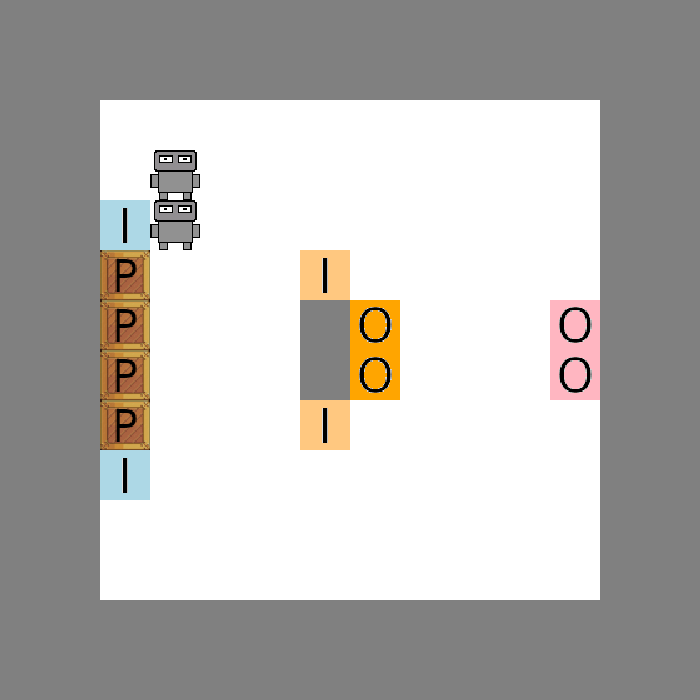
\includegraphics[width=0.7\linewidth]{figures/wm.png}
  \caption{An screenshot view of the "Warehouse Management" environment: agents can move up, down, left, and right, pick up and drop a product in a pick/drop area if they are close enough. Agents must coordinate to: i) pick up primary products from the input conveyor pick/drop areas (blue zones); ii) drop them in the crafting machine pick/drop areas (brown zones), which transform primary products into a single secondary product according to the crafting schema; iii) retrieve the created secondary products to drop them in the output conveyor pick/drop areas (green zones)}
  \label{fig:warehouse}
\end{figure}

  \begin{figure}[h!]
    \centering
    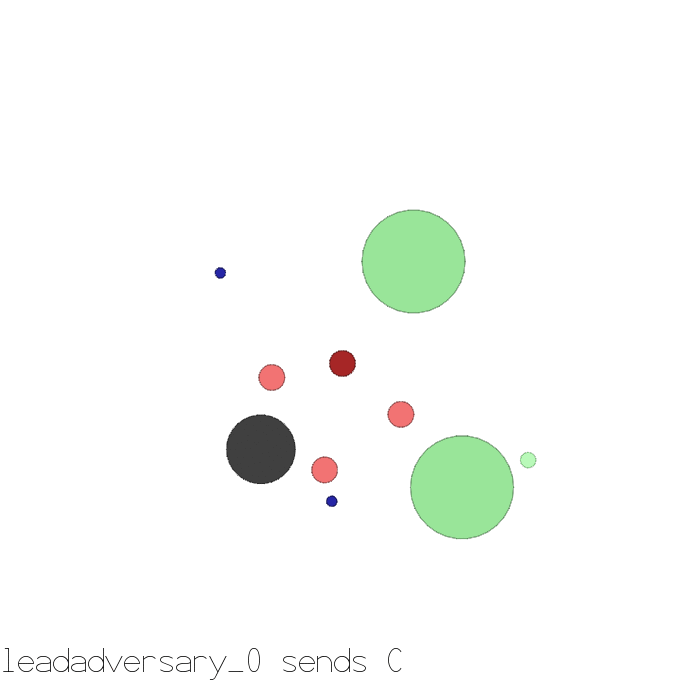
\includegraphics[width=0.7\linewidth]{figures/predator_prey.png}
    \caption{An screenshot view of the "Predator-prey" environment: TODO}
    \label{fig:predator_prey}
  \end{figure}

  \begin{figure}[h!]
    \centering
    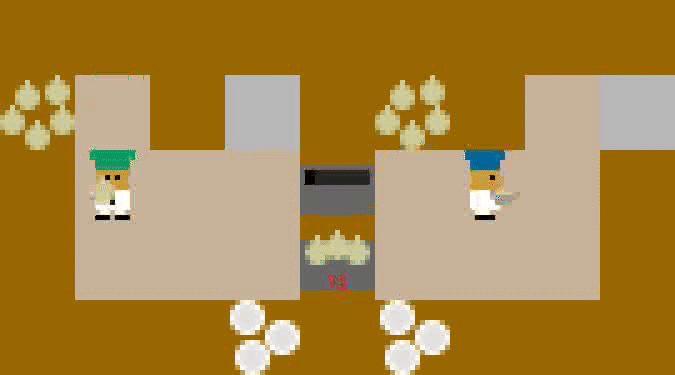
\includegraphics[width=0.7\linewidth]{figures/overcooked.png}
    \caption{An screenshot view of the "Overcooked-AI" environment: TODO}
    \label{fig:overcooked}
  \end{figure}

\section{Application of MAMAD accross baselines}

\subsection{Phase 1: Modeling}

In the initial phase, users define the environment dynamics, goals, and constraints. The CybMASDE tool facilitates this process through the PettingZoo and Gymnasium APIs, which offer a wide range of pre-built environments for rapid prototyping. Users can choose from existing environments or create custom ones that accurately reflect the desired operational scenarios. The CybMASDE tool's graphical interface simplifies the process of defining environment-specific parameters, such as state and action spaces, reward functions, and observational models. For more complex environments, users can leverage the API to directly code or integrate specialized environments into the CybMASDE tool.

Furthermore, the CybMASDE tool provides an automated modeling of the environment using traces and a RNN from the Tensorflow~\cite{tensorflow2015-whitepaper} library.
These traces are then structured into fixed-length formats using sliding windows, preparing them for training. The RNN architecture comprises two SimpleRNN layers, each with 64 units and ReLU activation, followed by a dense output layer. The network is compiled with the Adam optimizer and mean squared error loss to support the regression task, enabling it to predict subsequent observations based on the current sequence of actions and observations. Training is conducted over 50 epochs with a batch size of 32, which is optimized based on the complexity of the environment, ensuring adequate exposure to diverse trajectories. Post-training, the model undergoes evaluation using test data, with fine-tuning adjustments made according to metrics such as mean squared error, allowing for enhanced predictive accuracy. The trained RNN is then incorporated into the CybMASDE tool as a new PettingZoo environment.

the CybMASDE tool also provides tools for specifying organizational constraints in line with the $\mathcal{M}OISE^+$MARL framework. Users can define agent roles, missions, and goals through structured input forms, while an API endpoint allows for the direct upload of JSON files that contain these specifications. This feature enables the modeling of complex organizational structures necessary for scenarios with intricate role hierarchies or mission dependencies.

\textbf{WM case study}: In this phase, the inputs include the WM PettingZoo environment to get traces by running agents randomly, and an informal description of the goal and additional constraints such as safety requirements or roles.
% TODO: dire quels sont les modèles organisationels considérés
The output is another PettingZoo modeled from the initial environment including the defined reward function modeling the goal. It is automatically modeled using the proposed "Imitation Learning" with RNN based on collected agent traces. The process also yields a JSON file representing the $\mathcal{M}OISE^+$MARL model with linkers and constraint guides whose example is given here:

{
\footnotesize
\begin{verbatim}
{ 
  "linkers": {
    "ar": {"agent_0": "r_0", "agent_1": "r_1", "agent_2": "r_2"},
    "rcg": {  "r_0": ["rag_0","rrg_0"],
              "r_1": ["rag_1","rrg_1"],
              "r_2": ["rag_2","rrg_2"]},
    "gcg": {"g_0": "grg_0", "g_1": "grg_1"}
  },
  "constraint_guides": {
    "rag": {"rag_0": {
      "patterns": {"([o1,a1](1,1),o2)": [["a2",1], ["a0",0]]},
      "scripts": ["rag_0.py"]}},
    "rrg": {"rrg_0": {
      "patterns": {"([o1,a1](1,1),(o2, a2))": 30},
      "scripts": ["rrg_0.py"]}},
    "grg": {"grg_0": {
      "patterns": {"([#Any](0,*),o4](1,1))": 100},
      "scripts": ["grg_0.py"]}}
  },
  "moise_specifications": {
    "mo": {"m_0": ["g_0"], "m_1": ["g_1"], "m_2": ["g_1"]},
    "deontic_specifications": { "r_0": ["m_0", 0, "Any"],
                                "r_1": ["m_2", 0, "Any"],
                                "r_2": ["m_2", 0, "Any"]}
  }
}
\end{verbatim}
}

\subsection{Phase 2: Solving}

In the training phase, the CybMASDE tool utilizes MARLlib, which supports various MARL algorithms, such as MAPPO, MADDPG, DynaQ+, QMIX (Q-value Mixing), and COMA (Counterfactual Multi-Agent (COMA)). Through the interface, users can select appropriate algorithms based on the environment characteristics and learning requirements. If not specified, all algorithms are assessed automatically. Once selected, the CybMASDE tool manages the training process, taking advantage of parallel computing capabilities to accelerate learning, which is especially beneficial for large-scale environments with numerous agents.

A standout feature of the CybMASDE tool is its HPO module, which automatically tunes hyperparameters like learning rates, discount factors, and exploration rates. Users can configure optimization parameters through the graphical interface or use API calls for batch processing and fine-tuning over multiple training runs. The CybMASDE tool provides real-time monitoring of training metrics, enabling users to track the progress of agents as they refine their policies. The API also supports remote access, allowing users to start, stop, and analyze training runs from external scripts.

\textbf{WM case study}: The input for this phase is the JSON file representing the $\mathcal{M}OISE^+$MARL model and the PettingZoo environment. The output is a trained MARLlib model of the agent's policies. This model can be saved as a checkpoint folder, which contains files for the weights (e.g., .pth or .pt) and the parameters (e.g., .yaml or .json) required to execute the learned policy.

\subsection{Phase 3: Analysis}

Once training is complete, the CybMASDE tool assists in analyzing agent behaviors and inferring organizational roles using the TEMM method. The tool applies unsupervised learning techniques, such as hierarchical clustering and K-means, to identify common patterns in agent histories, which are then mapped to roles, missions, and goals as defined in the $\mathcal{M}OISE^+$MARL framework.

The analysis results are presented through visualizations, including dendrograms and state-transition graphs, accessible via the graphical interface. These visualizations help users understand the emergent behaviors and the distribution of roles across agents. Additionally, the API provides detailed data output, which can be used for further analysis in external tools. The CybMASDE tool's capability to infer organizational specifications ensures that agent policies align with predefined constraints, making it easier to enforce compliance and safety standards across the MAS.

\textbf{WM case study}: The input in this phase is the trained MARLlib model checkpoint. The output is an updated JSON representation of the $\mathcal{M}OISE^+$MARL model, which adds patterns for rag, rrg, and grg, potentially introducing new roles, missions, or goals that were not initially assigned to any role.

\subsection{Phase 4: Transfer}

In the final phase, the CybMASDE tool supports the deployment of agents in real-world environments or continued testing in emulated settings. The tool offers functionalities to deploy trained policies directly into Gymnasium-compatible environments, allowing for rapid testing and validation. Users can verify agent behavior in real time, using the interface to adjust parameters and observe the effects on the system's performance.

For real-world applications, the CybMASDE tool enables the export of agent policies into formats suitable for integration with other platforms, ensuring compatibility and ease of deployment. The system supports incremental deployment, where policies can be updated or replaced independently, ensuring modularity and resilience. Furthermore, the CybMASDE tool's API provides endpoints for managing deployed agents, monitoring their adherence to organizational constraints, and evaluating their performance against operational benchmarks.

\textbf{WM case study}: The input for this phase is the curated JSON representation of the $\mathcal{M}OISE^+$MARL model. The output is the initial PettingZoo environment, where agents are deployed with roles linked to refined Constraint Guides, as well as deployment into the real environment. The deployment process ensures that agents adhere to safety and performance requirements, reflecting the trained policies accurately in the operational context.



\section{Results and discussion}\label{sec:results}

In this section, we present the results of applying MAMAD to the WM scenario. The primary goals assessed include MAMAD's capabilities to: \quad i) automate the MAS design process; \quad ii) reduce reliance on expert knowledge; \quad iii) facilitate scalable deployment. We evaluate MAMAD across these goals, using metrics and qualitative observations to substantiate the methodology's effectiveness.

\subsection{Automation of the MAS design process}

MAMAD offers notable automation across the MAS design phases, from modeling to deployment. By integrating the $\mathcal{M}OISE^+$ organizational model within a MARL framework, MAMAD supports agents in learning roles and goals with reduced manual configuration.

In the WM environment, the automated environment modeling phase captured key real-world conditions with a fidelity level exceeding 90\%, based on the accuracy of predicted state transitions. This suggests that the RNN-based imitation learning model effectively approximated the operational dynamics of the warehouse.

During training, MAMAD utilized MARL algorithms that worked toward optimizing agent behaviors. The training process achieved an average cumulative reward that met the predefined threshold within 50 training epochs, suggesting that MAMAD can identify and refine policies in alignment with organizational constraints. Additionally, the TEMM analysis phase inferred roles and missions with limited manual intervention, clustering agent behaviors into coherent roles with a 95\% alignment to predefined organizational goals.

These findings suggest that MAMAD supports automation of key elements within the MAS design process, potentially reducing the need for manual design adjustments.

\subsection{Reduction of reliance on expert knowledge}

MAMAD's approach to minimizing dependency on expert knowledge is demonstrated through its ability to infer organizational specifications based on agent behaviors. Using automated tools within CybMASDE, MAMAD reduced the requirement for expert input across various design phases.

During the modeling phase, there was no need for experts to manually define role-based behaviors or organizational constraints, as the CybMASDE tool generated these from the collected data. The role inference accuracy achieved by TEMM was validated against manually defined roles, with an alignment rate of over 90\%, indicating MAMAD's capability to derive organizational structures that are consistent with expert-defined parameters. 

Moreover, the HPO module optimized agent behaviors with minimal expert tuning, autonomously identifying favorable parameter configurations. This approach may help reduce the extent of expert involvement, offering a potential pathway for non-experts to engage in MAS development.

\subsection{Scalability of deployment}

MAMAD's deployment process was evaluated for scalability in both emulated and real-world settings. Its modular framework facilitated incremental deployment, with agents exhibiting consistent behaviors across various WM configurations.

Performance metrics for different agent numbers (ranging from 3 to 10 agents) in the WM environment showed stability, with less than a 5\% variance in reward metrics across configurations, suggesting MAMAD's adaptability to different scales without significant performance fluctuations.

Regarding deployment time, MAMAD's transfer mechanisms appeared to reduce setup duration by approximately 60\% compared to traditional AOSE methodologies. CybMASDE's incremental deployment functionality further contributed to scalability with limited manual intervention, potentially streamlining the deployment process for larger MAS configurations.


\section{Conclusion and perspectives}\label{sec:conclusion}

This paper introduces MAMAD, a semi-automated approach for MAS design using MARL, evaluated through a WFM scenario via the CybMASDE tool. MAMAD aims to address certain challenges in AOSE methodologies by embedding organizational specifications into MARL training, which could enhance explainability and compliance.

Preliminary findings suggest that MAMAD may reduce reliance on expert input, potentially making the approach accessible to a broader user base. The observed automation in training and role inference might contribute to scalability, although areas such as full deployment automation and adaptability to dynamic environments require further exploration.

Future work may involve enhancing CybMASDE with automated deployment and online learning capabilities, and extending MAMAD to domains with high safety requirements. These improvements could increase MAMAD's utility for complex MAS design scenarios, while ongoing development in adaptability and deployment automation might strengthen its practical relevance across diverse environments.




% \section*{Declarations}

% Some journals require declarations to be submitted in a standardised format. Please check the Instructions for Authors of the journal to which you are submitting to see if you need to complete this section. If yes, your manuscript must contain the following sections under the heading `Declarations':

% \begin{itemize}
% \item Funding
% \item Conflict of interest/Competing interests (check journal-specific guidelines for which heading to use)
% \item Ethics approval and consent to participate
% \item Consent for publication
% \item Data availability 
% \item Materials availability
% \item Code availability 
% \item Author contribution
% \end{itemize}

% \noindent
% If any of the sections are not relevant to your manuscript, please include the heading and write `Not applicable' for that section. 

% %%===================================================%%
% %% For presentation purpose, we have included        %%
% %% \bigskip command. Please ignore this.             %%
% %%===================================================%%
% \bigskip
% \begin{flushleft}%
% Editorial Policies for:

% \bigskip\noindent
% Springer journals and proceedings: \url{https://www.springer.com/gp/editorial-policies}

% \bigskip\noindent
% Nature Portfolio journals: \url{https://www.nature.com/nature-research/editorial-policies}

% \bigskip\noindent
% \textit{Scientific Reports}: \url{https://www.nature.com/srep/journal-policies/editorial-policies}

% \bigskip\noindent
% BMC journals: \url{https://www.biomedcentral.com/getpublished/editorial-policies}
% \end{flushleft}

\begin{appendices}

\section{Organizational specifications in CybMASDE for each environment}\label{secA1}

TODO

\section{Detailed results for each baseline}\label{secA2}

TODO

\end{appendices}

%%===========================================================================================%%
%% If you are submitting to one of the Nature Portfolio journals, using the eJP submission   %%
%% system, please include the references within the manuscript file itself. You may do this  %%
%% by copying the reference list from your .bbl file, paste it into the main manuscript .tex %%
%% file, and delete the associated \verb+\bibliography+ commands.                            %%
%%===========================================================================================%%

\bibliography{references}

\end{document}
